%!TEX root = ../thesis.tex
%*******************************************************************************
%****************************** Third Chapter **********************************
%*******************************************************************************
\chapter{Genome-wide Meta-analysis of All-cause Perianal Disease}

% **************************** Define Graphics Path **************************
\ifpdf
    \graphicspath{{Chapter3/Figs/Raster/}{Chapter3/Figs/PDF/}{Chapter3/Figs/}}
\else
    \graphicspath{{Chapter3/Figs/Vector/}{Chapter3/Figs/}}
\fi

\section{Contributions}
UK Biobank phenotype and genotype data were obtained by Dr. Laura Fachal. Genotype quality control and principal component analysis were also performed by Dr. Laura Fachal. All the other analyses described here were performed by me. 
\section{Introduction}

In the previous chapter, I described the characteristics and genetic underpinning of perianal Crohn's disease. However, perianal disease (pAD) is not only associated with Crohn's disease. pAD encompasses a broader set of perianal manifestations such as perianal abscess, fissures, and fistulas.\\

Anal fissures are tears and/or ulcers in the perianal skin that cause sharp pain associated with defecation and rectal bleeding. They are classified as acute, lasting less than 6 weeks, or chronic. The etiology of anal fissures is still debated \cite{Beaty2016-yj}, but they are thought to be caused by trauma resulting from high anal canal pressure associated with constipation or diarrhea \cite{Mapel2014-wp}. Although recent population studies on the etiology of anal fissures are markedly lacking \cite{Mapel2014-wp}, a number of studies conducted between 1977 and 1983 found that chronic constipation accompanied fissures in only 25\% of patients while diarrhea accounted for less than 7\% \cite{Keighley2018-iy,McDonald1983-cs,Lock1977-go}. Anal fissures are conservatively treated with dietary and lifestyle modifications, analgesics, and fiber supplements \cite{nice_analfiss}. Anal fistula is a more serious perianal manifestation of pAD. An anal fistula is defined as an abormal communication between the anal canal and the perianal skin \cite{Sneider2013-qd}. It is characterised by pain, rectal discharge and bleeding, and causes significant lifestyle difficulties for patients \cite{Mei2019-ds}. The incidence of perianal fistulas varies per country, and a recent study in four European countries found that it ranges from 1.2 to 2.8 per 10,000 per year \cite{Zanotti2007-mb}, but its incidence is likely underestimated \cite{Eberspacher2022-sp}. Moreover, little is known about the pathophyiology of anal fistulas. Cryptograndualr fistulisation, a theory proposed by Parks in 1961 \cite{Parks1961-pe,Wlodarczyk2021-kh}, is the most accepted pathophysiological account for the origin of anal fistulas. Accoring to the cryptograndular theory, anal fistuls start as an inflammatory process in the proctodeal glands whose ducts extend to connect the perianal skin to the anal canal. Crohn's disease, tuberculosis \cite{Dudukgian2011-is}, ratiotherapy \cite{Johnston2003-jr}, sexually transmitted diseases \cite{Assi2014-at} and malignancy can contribute to these initial inflammatory process that resultin  anal fistula formation. However, over 90\% of cases remain idiopathic \cite{Simpson2012-gi}. Management of anal fistula depends on its type, extension, and underlying cause, but the end goal of all treatments is the complete drainage of abscess, and fistula healing while preserving anal sphincter function and continence. The management plan is typically decided based on a combined clinical, radiological and/or endoscopic assessment. Surgical options of fistula management include fistulectomy, the complete excision of the fistula tract, and fistuolotomy, in which the fistula is laid open and allowed to heal. Surgical procedures that preserve anal function such as fistolotomy with sphincter reconstruction have emerged in the last 30 years as a particularly effective method of treating anal fistulas, with lower incontinence and recurrence rates compared to fistulectomy \cite{Arroyo2012-qa,Jain2012-or}. \\

Despite recent advances in the management of pAD, little is known about the biological and pathophysiological processes that lead to anal fissure and fistula formation. Despite the overall consensus on the cryptoglandular theory, it is unclear if some individuals are at higher risk of developing pAD due to their genetic predisposition. Genome-wide association studies (GWAS) have significantly improved our understanding of the genetic factors underlying several complex diseases as well as the biological pathways implicated by disease-associated genetic variants. In the last 15 years, a typical GWAS required extensive coordination between researchers, clinicians and recruitment centres to construct case-control cohorts to study a particular disease or trait of interest. In recent years, efforts to build various national biobanks where genetic, and phenotypic data are available for hundreds of thousands of participants has significantly improved our ability to conduct GWAS of previously understudied diseases and traits. Their large sample sizes have made it possible to carry out GWAS of thousands of binary and continuous traits and diseases, including relatively uncommon diseases. \\

Recruitment for the UK Biobank (UKBB) started in 2006, and has so far collected genotypic, biomarker and clinical data from electronic health records as well as blood and urine samples from over 500,000 participants \cite{ukbb_showcase}. The UKBB queries electronic health records for various types of data including deaths, cancer registrations, and hospital inpatient episodes. Electronic health records data are provided by external sources. Upon receipt of the data, a multi-step approach is followed, where received data is subjected to further pre-processing and quality checks to ensure its alignment with the UKBB data dictionary, and that it does not contain any ambiguities. The data is then consolidated into a central UKBB database and made available to researchers \cite{ukbb_ehr}.\\

FinnGen is another example of national biobanks that has made GWAS for various traits and diseases more feasible. FinnGen started in 2017 as a public-private partnership between several public Finnish institutions and thirteen international pharmaceutical companies \cite{finngen_forresearchers}. Importantly, FinnGen restricts access to individual-lvel data to approved researchers only. However, summary statistics data from GWAS analyses are made publicly available. In its latest release (data freeze 9), GWAS are available for over 2,200 binary endpoints from 377,277 individuals \cite{finngen_aboutdf9}. \\

The UKBB and FinnGen use slightly different clinical coding systems to register clinical data. The UKBB uses the International Classification of Disease (ICD), a hierarchical clinical framework that organises clinical diagnoses in a tree-like structure. Different groups of diseases are organised in alphabetical chapters and particular diseases within each chapter are given a numeric value (e.g. chapter K contains digestive system disorders and K60 indicates anal fissure and fistula). Further detailed diagnosis subtypes are nested within each alphanumeric code up to four levels of resolution \cite{icd10_levels}. However, the UKBB only records up to two levels of resolution (e.g. K50.0 indicates Crohn's disease of the small intestine). FinnGen, on the other hand uses an expert-curated set of endpoints that are largely parallel to ICD-10 codes. These endpoints are designed to accommodate inclusion and exclusion criteria relevant for GWAS analyses \cite{finngen_endpoints}. Despite these differences, both resources are valuable for studying pAD. \\

In this chapter, I will describe a pAD GWAS I performed in the UKBB to map pAD-associated genetic variants and I will describe the post-GWAS quality checks I carried out to ensure the validity of genome-wide significant loci. Additionally, I will outline how I used summary statistics from the FinnGen GWAS both as a replication dataset and as a constituent cohort in a pAD meta-analysis I performed between the UKBB and FinnGen cohorts. Finally, I will describe two follow-up analyses that I performed to better understand the effects of pAD-associated variants on haemorrhoids, a closely-related disease, and identify effector genes at these loci.

\section{Methods}
\subsection{UKBB sample preparation and data access}
Hospital inpatient episode data and genotyped and imputed data were obtained under UK Biobank Application 45669. UKBB participants were genotyped using either UK Biobank Axiom Array \cite{ukbbaxiom_array} or the Affymetrix UK
BiLEVE Axiom array \cite{ukbbbelieve_array}. Sample processing, genotyping and quality control were performed at the UK Biobank, Affymetrix and the Wellcome Trust Centre for Human Genetics \cite{ukbb_sample_processing}. The imputation process has been previously described \cite{Bycroft2018-fj} and consists of imputing directly genotype data to the Haplotype Reference Consortium (HRC) and UK10K, resulting in 96 million variants. Imputed data was obtained as BGEN v1.2 files \cite{Band2018-tv}. 
\subsection{Defining pAD case control cohorts}
% With every inpatient visit, patients receive a primary and secondary diagnosis. These diagnoses are recorded using a hierarchical clinical diagnosis framework known as The International Classification of Diseases (ICD) \cite{Hirsch2016-mw}. ICD is a hierarchical framework whereby each medical diagnosis is given an alphanumeric code, and all sub-classifications of any given diagnosis are nested within it. For example, K50 codes for Crohn's disease, while K50.1 codes for Crohn's disease in the large intestine. In this chapter, I will refer to the main ICD codes as "level 1 codes" and their sub-classifications "level 2 codes". The level 1 code for perianal involvement is K60 (K60: Fissure and fistula of the anal and rectal regions)

% To understand the genetic architecture of perianal involvement in the general population, I performed a GWAS analysis between all-cause peri-anal disease (pAD) and healthy individuals in the UKBB. 

\subsubsection{Case inclusion criteria}
To define the case cohort, I identified all individuals with ICD-10 code K60 or ICD-9 code 565. In total, 5,257 UKBB participants had at least a single visit where they received either a primary or secondary pAD diagnosis or its corresponding ICD-9 code ("anal fissure and fistula"; 565). Six level-2 codes are nested within K60, representing two broad categories of pAD: fissures and fistulas. Three codes are used for acute and chronic fissures and three codes for acute and chronic fistulas. 92\% of patients (4,858) presented with either K60.1, K60.2 or K60.3 ("chronic anal fissure", "anal fissure, unspecified" and "anal fistula", respectively; Table \ref{table:ukbb_level2_nums}).


\subsubsection{Control exclusion criteria}
To avoid contamination of controls with lower digestive tract disorders that may be true pAD cases that were incorrectly diagnosed, I applied a set of control exclusion criteria. Specifically, I excluded from the control set any individuals who had an ICD-10 hospital diagnosis of K55-K64 or their corresponding ICD-9 codes as outlined in Table \ref{table:ukbb_ctrl_excl_criteria} (collectively grouped as "Other diseases of intestines" in ICD). These ICD codes cover disorders with symptoms that may resemble pAD symptoms upon presentation, and include ano-rectal bleeding (K55 vascular disorders of the intestine, K57 diverticular disease of intestine and K64 Haemorrhoids and perianal venous thrombosis), or a change in bowel habits (K56 Paralytic ileus and K58 Irritable bowel syndrome), perianal fistula or abscess (K60 fissure and fistula of the anal region and K61 abscess of the anal and rectal region), any ano-rectal abnormalities (K62), or proximal fistulas or abscesses (K63). In total, I excluded 128,319 individuals from the control cohort (26.7\%), resulting in 353,437 controls (per-code number of individuals in Table \ref{table:ukbb_level2_nums}).



\begin{table}[H]
  \centering
  \caption{Number of UKB participant with with a primary or secondary diagnosis for each K60 level 2 code. K60.0=Acute Anal Fissure; K60.1=Chronic Anal Fissure; K60.2=Anal Fissure; unspecified; K60.3=Anal Fistula; K60.4=Rectal Fistula; K60.5= Anorectal Fistula}
  \label{table:ukbb_level2_nums}
  \begin{tabular}{|l|l|l|l|l|l|l|}
  \hline
  ICD-10 code           & K60.0  & K60.1  & K60.2  & K60.3 & K60.4 & K60.5\\ \hline
  Number of individuals & 144                      & 788                        & 2,624                           & 1,954              & 76                   & 122                     \\ \hline
  \end{tabular}
  \end{table}




\begin{table}[H]
  \caption{pAD control set exclusion criteria. All ICD-10 codes had corresponding ICD-9 codes except K56 K62 and K63. For those, ICD-9 codes were obtained manually by inspecting level-2 ICD-10 codes and searching for their corresponding level-2 ICD-9 codes.}
  \label{table:ukbb_ctrl_excl_criteria}
  \begin{tabular}{|p{0.1\linewidth}|p{0.2\linewidth}|p{0.2\linewidth}|p{0.3\linewidth}|p{0.1\linewidth}|}
  \hline
  ICD-10 code & ICD-10 meaning                                            & ICD-9 code                          & ICD-9 meaning     & N                                                                                                                                                          \\ \hline
  K55         & Vascular disorders of intestine                           & 557                                 & Vascular insufficiency of intestine       & 2923                                                                                                                                  \\ \hline
  K56         & Paralytic ileus and intestinal obstruction without hernia & 5600, 5601, 5602, 5603, 5608A, 5608, 5609 & Intussusception, Paralytic ileus, Volvulus, Impaction of intestine,Other specified intestinal obstruction, Unspecified intestinal obstruction & 9257                              \\ \hline
  K57         & Diverticular disease of intestine                         & 562                                 & Diverticula of intestine              &     61519                                                                                                                                  \\ \hline
  K58         & Irritable bowel syndrome                                  & 5641                                & Irritable bowel syndrome          & 12418                                                                                                                                          \\ \hline
  K59         & Other functional intestinal disorders                     & 564                                 & Functional digestive disorders not elsewhere classified      & 30087                                                                                                               \\ \hline
  K60         & Fissure and fistula of anal and rectal regions            & 565                                 & Anal fissure and fistula     & 5079                                                                                                                                               \\ \hline
  K61         & Abscess of anal and rectal regions                        & 566                                 & Abscess of anal and rectal regions              &     2178                                                                                                                        \\ \hline
  K62         & Other diseases of anus and rectum                         & 5690, 5691, 5692, 5693, 5694            & Anal and rectal polyp, Rectal prolapse, Stenosis of rectum and anus, Hemorrhage of rectum and anus, Other specified disorders of rectum and anus            & 39191                \\ \hline
  K63         & Other diseases of intestine                               & 5695, 5696, 5697, 5698, 5699            & Abscess of intestine, Colostomy and enterostomy complications, Complications of intestinal pouch, Other specified disorders of intestine, Unspecified disorder of intestine & 33307 \\ \hline
  K64         & Hemorrhoids and perianal venous thrombosis                & 455                                 & Hemorrhoids & 19060\\ \hline

  \end{tabular}
  \end{table}
\subsection{ICD code enrichment in pAD cases versus controls}
The availability of a large number of clinical diagnoses and phenotypes for UKB participants enables a thorough characterisation of the pAD case cohort. I aimed to understand the cohort composition by identifying which ICD-10 codes are enriched in cases versus controls. For each ICD-10 code, I compared the prevalence in pAD cases versus controls, and I formally tested the enrichment of 1,693 codes using Fisher's exact test. For this test, I did not apply the control exclusion criteria outlined in Table \ref{table:ukbb_ctrl_excl_criteria}.
\subsection{UKBB genotype quality control}
Genotyping array data from the UK Biobank dataset underwent quality control as part of the International IBD Genetics Consortium GWAS that is being undertaken in the laboratory, which resulted in 419,871 variants being retained. QC was performed using a combination of PLINK (v1.9 and v2) \cite{Purcell2007-mu}, bcftools (v1.16) \cite{Li2011-td}, and KING (v2.2.4) \cite{king-software}.  Variants that met the following criteria were excluded: 
\begin{itemize}
  \item Low call rate (<0.95 for variants with minor allele frequency (MAF) $>$ 0.01 or $<$ 0.98 for variants with MAF $\leq$ 0.01).
  \item Significant difference in genotype call rate (P-value $< 10^{-4}$) between IBD cases and controls.
  \item Large allele frequency (AF) differences between UKBB and Gnomad (Non-Finnish Europeans), or TOPMed (global) using the following formula: $\frac{(P_{1}-P_{0})^{2}}{(P_{1}+P_{0})(2-P_{1}-P_{0})} > \epsilon$, where $\epsilon=0.025$ or $0.125$, for Gnomad and TOPmed respectively,  $P_{0}$ is the minor allele frequency (MAF) in Gnomad or TOPMed and $P_{1}$ is the UKBB MAF. 
\end{itemize}

Genotypic principal components (PC) were estimated for all participants, using a set of genotyped variants that were also available in the 1000 Genomes Project (1000GP; excluding variants associated with IBD susceptibility (P-value < $10^{-4}$), and variants in long LD regions (as defined in \cite{plink_high_ld}). This final list of variants was pruned with the following parameters: window size = 50 kbp; step size = 5; $R^{2}$ = 0.2. PCs were then projected to 1000GP PCs. Samples within the European ancestry group were retained for the subsequent analyses. 



\subsection{UKBB GWAS using REGENIE}
All genome-wide association analyses were performed using REGENIE v3.2.5 \cite{Mbatchou2021-qm} following a 2-step approach. This approach achieves higher computational efficiency compared to linear mixed model, which are normally used in GWAS methods to account for cryptic relatedness. Briefly, in step 1, a whole-genome regression model is fitted using a subset of high-quality genome-wide variants in order to estimate a set of genome-wide predictors that capture a large fraction of phenotypic variance. These predictors are then used in step 2 in a single-variant association testing model, where a larger set of variants of interest are tested for association. I used post-QC genotyped variants in step 1 as recommended by REGENIE documentation (N=419,871), and both genotyped and imputed variants in step 2, testing all autosomal chromosomes (N=9,705,089). Additionally, I enabled a Firth correction of effect sizes for all variants with P-value < 0.01 in order to account for the case-control imbalance in the pAD cohort (\Verb+--firth --approx --pThresh 0.01+). The Firth test corrects biased effect sizes and P-values obtained from highly unbalanced case-control designs, where such an imbalance causes unreliable P-values, inflating Type I error. Approximate Firth logistic regression is a variant of the Firth test that is more computationally tractable and is implemented in REGENIE. \\

With the pAD case control cohort defined above, I used REGENIE to perform a pAD GWAS with White British UKBB participants \cite{Mbatchou2021-qm}. In addition to genotype QC described earlier, I  excluded individuals with missing genotypes or with discordant reported and genetically-inferred sex. After this filtering a total of 4,606 pAD cases and 332,234 pAD controls remained (see Methods for genotype data quality control and imputation). In order to account for cryptic population stratification, I used 10 European-ancestry genotypic principal components, as well as sex and genotyping array as covariates in the REGENIE model. After filtering out variants with low imputation quality (INFO < 0.4) and minor allele frequency (MAF) < 0.01, a total of 9,705,089 variants were tested. After running REGENIE, I found that the summary statistics exhibited moderate genomic inflation (median $\chi^{2}=0.48$; $\lambda_{GC}=1.06$). 
%Although $\lambda_{GC}$ values up to 1.05 are considered acceptable, higher values can be expected in GWAS with large sample sizes \cite{Price2010-zb}. In the next two sections, I will describe how I identified genome-wide significant loci, and the further quality checks I performed to ensure their validity. 
  

\subsection{LD calculation from 1000GP}
Reference LD panels obtained from the 1000 Genomes Project High Coverage project \cite{1000gphc} were used for different analysis, including genome-wide loci identification using LD clumping, and post-GWAS checks to study the relationship between LD and association strength at genome-wide significant loci. $R^{2}$ values were calculated between the index variant and all variants in each locus (loci were defined using LD clumping as described in the next section). I downloaded VCFs from the 1000GP high coverage and used PLINK v1.9 to compute LD between all variants and the index variant at each locus. For each GWAS check, I used unrelated individuals assigned to the relevant reference population: NFE and GBR for UKBB and FE for Finngen (N=426, 99 and 90 respectively). Only one sample was retained from the trios found in 1000GP. Relevant samples were included in the LD calculation using the following PLINK command:
\begin{verbatim}
  plink --r2 --keep EUR.samples --ld-window-r2 0 
\end{verbatim}

\subsection{Defining genome-wide significant loci in UKBB}
I defined genome-wide significant loci from the UKBB pAD GWAS summary statistics using PLINK v1.9 via a clumping procedure. Briefly, LD clumping identifies the most significant variant in a user-defined window to represent each locus (termed index variant). It then proceeds to define the locus boundaries by clumping neighbouring correlated variants. Specifically, any variants within the predefined window that are correlated with the index variant are considered to belong to the same locus represented by the index variant (i.e. variants in high LD). I used VCFs downloaded from the 1000GP, which are used to compute LD, and set a maximum P-value of $5\times10^{-8}$ for defining a genome-wide significant locus, with default values for the rest of the parameters: variants with $R^{2}$ < 0.5, variants outside a window of 250 kbp, or variants that have a P-value > 0.01 are not clumped with the index variant.
\begin{verbatim}
  plink --clump-p1 0.00000005 --clump-r2 0.50 --clump-kb 250 
  --clump-p2 0.01
\end{verbatim}

PLINK outputs each locus' index variant along with any variants that meet the clumping criteria outlined above. I then defined each locus' boundaries by sorting the clumped variants within each locus according to their genomic location: the most downstream variant defined the 5' boundary and the most upstream variant defined the 3' boundary. 

\subsection{Finngen summary statistics preprocessing}
Publicly available FinnGen GWAS summary statistics (data freeze 7) were downloaded from the FinnGen results website \Verb+finngen.fi/en/access_results+. Similar to UKBB, variants with MAF < 0.01 were removed, but imputation quality information were not available, so I was not able to filter out variants with low imputation quality. The association summary statistics showed evidence of moderate genomic inflation ($\lambda_{GC}$=1.089). I used LD clumping with a 1000GP-derived FE LD reference panel to identify genome-wide significant loci. 

\subsection{Meta-analysis of UKBB and Finngen}
I used METAL to perform the meta-analysis between UKBB and FinnGen GWAS summary statistics.  METAL can perform fixed-effects meta-analysis using one of two different well-established schemes: P-values and effective sample size, or effect sizes and standard errors. The P-value scheme is implemented to enable meta-analysis of GWAS summary statistics that do not report the effect allele, while the effect sizes scheme can be used when each variant's effect size and effect allele are reported. Both my UKBB analysis and FinnGen's summary statistics report the effect allele, so I used the effect size scheme of METAL (\Verb+SCHEME STDERR+). \\

% Moreover, METAL automatically aligns any variants that may be flipped between the meta-analysed summary statistics. METAL also enables filtering of variants to be meta-analysed based on their allele frequencies, which was not necessary since I previously filter out variants with MAF < 0.01 in each summary statistics file. Finally, given the differences in allele frequencies, and potential subpopulation stratification between the FinnGen and UKBB GWAS, I enabled a METAL option to correct genomic inflation before performing the meta-analysis (\Verb+GENOMICCONTROL ON+) as recommended in METAL's documentation website. There was no evidence of genomic inflation in the meta-analysed summary statistics ($\lambda_{GC}$=1.024).\\


After filtering out variants with MAF < 0.01 and with low imputation score (INFO < 0.4), the two GWAS summary statistics had an intersection of 7,663,827 variants and a total of 11,096,129 variants across the two cohorts. Of these, 2,041,145 variants were specific to UKBB and 1,390,527 were specific to FinnGen. Given that 31\% of variants were unique to one of the two GWAS, I did not remove them from their respective summary statistics file. It is important to note, however, that this choice may favour variants that are available in both studies. Additionally, I enabled METAL's \Verb+GENOMICCONTROL ON+ option to correct genomic inflation in each of the two summary statistics before performing the meta-analysis. The resulting meta-analysed summary statistics showed no evidence of genomic inflation ($\lambda_{GC}$=1.02).\\

For each variant, METAL outputs the effect allele, meta-analysed effect size, standard error, and P-value. After performing meta-analyses, it is important to compare the effect sizes between the meta-analysed cohorts. Comparison of both the direction and magnitude of effect sizes gives an indication on how similar the estimated effects of meta-analysed genetic variants are, which is an import post-GWAS quality control check. To formally test this, METAL uses Cochran's Q test to test for effect size heterogeneity. Cochran's Q test asseses two or more effect size estimates and their corresponding standard errors and reports a $\chi^{2}$ statistic that quantifies the deviation from the null hypothesis that the meta-analysed effect sizes are similar. Depending on the number of meta-analysed studies (in this case 2), a P-value is derived from a theoretical $\chi^{2}$ distribution with $N-1$ degrees of freedom, where N is the number of meta-analysed studies (heterogeneity of effect P-value $P_{het}$). I used $P_{het}$ to test if index variants at genome-wide significant loci demonstrate heterogeity of effect size between the two cohorts. To account for multiple index variants being tested, I set a Bonferroni-corrected P-value threshold for rejecting the null hypothesis that the effect sizes are similar between the two studies (P-value < $\frac{0.05}{k}$, where $k$ is the number index variants tested).


\subsection{Defining genome-wide significant loci in the UKBB/FinnGen meta-analysis}
Meta-analysis associations are derived from two different populations with different LD structures (NFE and FE). 
For these associations, a  representative LD reference panel that captures the true underlying LD pattern in the meta-analysis is not easy to obtain because LD will be dependent on the contribution of each population to the association signal. However, an LD reference panel is needed both to define genome-wide significant loci based on LD clumping, but also to perform post-GWAS checks. To this end, I identified genome-wide significant loci similar to UKBB and FinnGen, except that I performed LD clumping of the meta-analysis genome-wide significant loci once with an LD reference panel derived from NFE in 1000GP, and once with an LD reference panel derived from FE in 1000GP. Both LD clumping procedures identified the same 18 genome-wide significant loci, but their boundaries differed slighly. I defined consensus loci boundaries as the union of loci boundaries defined by NFE- and FE-based LD clumping. \\

\subsection{Quality control of meta-analysis genome-wide significant loci}
For all 18 genome-wide significant loci defined via the initial LD clumping procedure, I investigated the LD friends of each index variant. Specifically, for each index variant, I checked if the P-values of its LD friends decay linearly with their LD values with the index variant. In a meta-analysis between different subpopulations, it is important to ensure that P-values match expectation under LD  in all the constituent cohorts. I therefore computed the correlation between P-values and LD in both NFE and FE for all 18 loci. Six loci showed that the index variant had no LD friends in NFE or FE, or that there was weak or non-existent correlation beween P-values and LD of the index variant's LD friends in NFE or FE (Pearson correlation coefficient between $-log_{10}(P)$ adn ($R^{2}$ $\rho$ < 0.2). I removed these six loci from all downstream analysis.









\subsection{Genetic correlation analysis}
Genetic correlation analysis is commonly employed to understand the genetic similarities between two phenotypes or diseases of interest. I used genetic correlation to understand the overall genetic similarity between pAD and haemorrhoids. Linkage disequillibrium score regression is a common method to compute genome-wide genetic correlation,(LDSC \cite{Bulik-Sullivan2015-fk}) as it leverages association summary statistics between a pair of traits to compute a genetic correlation estimate ($r_{g}$). The availability of GWAS summary statistics for large numbers of traits and diseases makes genetic correlation a feasible exploratory analysis to discover genetic similarities between traits.\\

The fundamental concept of LDSC is that there is a linear relationship between the Z-score product ($z_{1}z_{2}$) and the LD score of SNPs, where LD score is defined as the sum of $R^{2}$ values for all SNP in a pre-defined windown (the default is 1 cM) \cite{Bulik-Sullivan2015-ts}. The rationale behind this relationship is that SNPs with a higher LD score are more likely to tag the causal variant at each locus, and will therefore have a larger $z_{1}z_{2}$ value. Regressing the LD score for all SNPs can give an estimate of the overall genetic covariance between two traits. Specifically, the regression slope quantifies the gentic covariance, which can then be normalised by the sample sizes of the two traits and the number of SNPs to obtain a genetic correlation estimate between the two traits ($r_{g}$).\\

The accuracy of $r_{g}$ rests on the assumption that the GWAS population matches the population from which LD scores are derived. By default, LD scores are provided by LDSC, which are computed from the HapMap3 European-ancestry reference panel \cite{hapmap}. It is also important to note that although $r_{g}$ is a genome-wide measure, its computation is based on a predefined set of SNPs. The estimation of $r_{g}$ is based on a set of high-quality common SNPs in HapMap3, which is also provided by LDSC (MAF $\geq$ 0.05; N=1,217,312).

\subsubsection{Genetic correlation between pAD and haemorrhoids}
I used LDSC to compute $r_{g}$ between my pAD meta-analysis and two haemorrhoids GWASes (Zheng et al. 2021 \cite{Zheng2021-ss} and the Pan-UKBB GWAS: \Verb+pan.ukbb.broadinstitute.org/+). I downloaded the Zheng et al. 2021 summary statistics via the GWAS catalogue website (study accession: GCST90014033; $N_{cases}$=218,920; $N_{controls}$=725,213). Since the Pan-UKBB performed the haemorrhoids GWAS using different ancestries, I used the summary statistics from the European-ancestry GWAS only (ICD-10 code: I84; $N_{cases}$=26,348; $N_{controls}$=394,183). \\

After downloading the two haemorrhoids summary statistics, I preprocessed both of them using the LDSC script \Verb+munge_sumstats.py+. The script filters the SNPs and aligns their alleles to the HapMap3 SNP list using the flag \Verb+--merge_alleles hm3.snplist+. This script also takes as input a signed summary statistic column which I provided using the flag \Verb+--signed-sumstats effect_size,0+, where the first argument specifies the column name (effect size column) and the second argument specifies the expected value of the signed summary statistic. Each of the two "munged" summary statistics files were then provided as input to the \Verb+ldsc.py --rg+, along with the pAD summary statistics file, and $r_{g}$ is then computed between pAD and each of the two haemorrhoids GWASes. 


\subsection{Colocalisation analysis}
In order to link the meta-analysis genome-wide significant loci to effector genes, I performed statistical colocalisation with a set of expression and splicing QTLs from the Genotype Expression Project (GTEx v8). Colocalisation analysis is a statistical approach that uses summary statistics from two association studies in order to make an inference whether the two association signal are likely to be driven by a shared causal variant. In this regard, five different hypothesis regarding the relationship between the two association signals are tested:
\begin{itemize}
  \item $H_{0}$: none of the two signals are associated with their corresponding traits
  \item $H_{1}$: only the first signal is associated with its corresponding trait
  \item $H_{2}$: only the second signal is associated with it corresponding trait
  \item $H_{3}$: the two signals are associated with their corresponding traits, with different underlying genetic variants
  \item $H_{4}$: the two signals are associated with their corresponding traits, and share a single underlying genetic variant.
\end{itemize}
Certainty about each of these hypotheses is quantified as a posterior probability. Therefore, colocalisation analysis outputs four different posterior probabilities: $PP_{0}$, $PP_{1}$, $PP_{2}$, $PP_{3}$, and $PP_{4}$. Statistical colocalisation is implemented in the R package \Verb+coloc v5.1.2+.

To maximise the ability of \Verb+coloc+ to identify effector genes, I downloaded summary statistics from GTEx v8, a large compendium of expression and splicing quantitative trait loci (eQTLs and sQTLs) mapped from RNA-seq samples obtained from 49 human tissues, ranging in sample sizes from 73-706 individuals. eQTLs and sQTLs were mapped in a 1mbp window centred around the transcript start site (TSS) of each gene (cis-eQTLs and cis-sQTLs) using genotyped or imputed variants with MAF $\geq$ 0.01.

Within each of the meta-analysis genome-wide significant loci, I identified a list of genes and splice junctions for eQTL and sQTL colocalisation, respectively. To achieve this, for each locus I defined a 1 mbp window around the index variant at each locus, and created a set of genes and splice junctions whose respective TSS are located within this window. Next, I performed colocalisation analysis between the meta-analysis summary statistics and each eQTLs and sQTLs summary statistics for each gene in the window. I used the \Verb+coloc.abf()+, which takes as input effect sizes and standard errors of each variant from the meta-analysis and gene or splice junction being tested. Importantly, \Verb+coloc.abf()+ does not require the effect sizes to be aligned to the same effect allele, as the Bayes Factor calculation implemented in \Verb+coloc+ relies on the $Z^{2}$ statistic to compute the posterior probabilities. Finally, I used the default priors implemented in \Verb+coloc.abf()+: prior probability a SNP is associated with pAD=$10^{-4}$, prior probability a SNP is associated with the eQTL/sQTL=$10^{-4}$.

\begin{table}[H]

  \caption{Number of eQTL and sQTL genes tested for colocalisation across all GTEx v8 tissues. All genes and splice junctions in a 1mbp around each index variant were tested.}
  \centering
  \begin{tabular}[t]{|l|r|r|}
  \hline
  Index variant & Number of tested eQTL genes & Number of tested sQTL genes\\
  \hline
  3:53034026\_C\_T & 41 & 18\\
  \hline
  5:64868326\_TTTC\_T & 13 & 4\\
  \hline
  6:1775202\_G\_A & 12 & 5\\
  \hline
  6:31121854\_C\_T & 89 & 45\\
  \hline
  6:31253340\_T\_C & 98 & 50\\
  \hline
  6:133260944\_G\_A & 18 & 7\\
  \hline
  7:2524404\_G\_A & 21 & 13\\
  \hline
  8:70735125\_A\_G & 15 & 6\\
  \hline
  8:70993166\_AAGTT\_A & 10 & 6\\
  \hline
  9:22124505\_A\_T & 19 & 5\\
  \hline
  11:10356352\_C\_A & 20 & 11\\
  \hline
  12:114235969\_T\_C & 18 & 10\\
  \hline
  \end{tabular}
  \end{table}



\section{Results}



  \subsection{pAD cases are enriched in multiple disorders compared to pAD controls}\label{section:pheno_enrich}


  In order to understand the composition of the pAD case cohort, I tested the enrichment of 1,693 ICD-10 codes in pAD cases versus controls. Overall, the tested enrichment odds ratio were inflated (median odds ratio=1.36), likely as a consequence of sampling a disease cohort within a healthy population cohort. In total, 198 codes were significantly enriched among cases versus controls (Fisher's exact  P-value < $3\times10^{-5}$; top 20 enriched ICD-10 codes are shown in Figure \ref{fig:pheno_enrich}).  Within digestive systems disorders, ICD-10 code K61 (abscess of anal and rectal regions), followed by K50 (Crohn's disease) were the most significantly enriched (log odds ratio=4.04 and 1.96 respectively). This is expected as many perianal fistulas start as abscess of the perianal region and later extend to form a fistula connecting the anorectal canal to the perianal skin \cite{abscess_fist}, and perianal fissures and fistulas are known subphenotypes of CD \cite{Marzo2015-wf}. Other examples indlude K57 (Diverticular disease of the intestine; log odds ratio=0.74; P-value=$1.2\times10^{-87}$), which is also a known cause of pAD \cite{div_pad}. Among non-digestive codes, haemorrhoids (I84) was the most significantly enriched diagnosis (P-value=$6\times10^{-98}$; 38\% in pAD cases versus 6\% in controls; log odds ratio=2.3). This enrichment could indicate a shared pathogenesis between haemorrhoids and pAD. However, it could also be due to a higher likelihood of diagnosing haemorrhoids in patients with more serious ano-rectal disorders such as pAD, compared to the general population where haemorrhoids patients with no other ano-rectal manifestations are less likely to seek medical advice, and may therefore remain undiagnosed. \\

    %To understand which groups of disorders were most enriched in pAD cases, I counted the number of enriched disorders within each ICD-10 code categry. I found that five groups had > 10 enriched ICD codes. The largest number of enriched codes belonged to: "Symptoms, signs and abnormal clinical and laboratory findings, not elsewhere classified (R00-R99)" (36 codes), followed by "Diseases of the digestive system (K00-K95)" (34 codes), "Diseases of the genitourinary system (N00-N99)" (22 codes), "Diseases of the musculoskeletal system and connective tissue (M00-M99)" (20 codes), and "Diseases of the skin and subcutaneous tissue (L00-L99)" (15 codes), "Diseases of the circulatory system (I00-I99)" (13 codes).\\
% However, not all enrichments were expected. For example, pAD cases were 1.6 more likely to be diagnosed with gonorthrosis, a gradual erosion of the knee cartialge (P-value=$1.3\times10^{-22}$; odds ratio=1.6; prevalence in pAD cases is 12\% versus 8\% in controls). A clinical report has previously described chronic arthritis as an "unusual complication" of poorly treated anal fistulas. However, it remains to be answered if such higher prevalence in UKBB can be attributed to poor management or complications, or if it suggests a musculoskeletal or connective tissue pathology underlying fissures and fistulas. 



\begin{figure}[H] 
  \centering    
  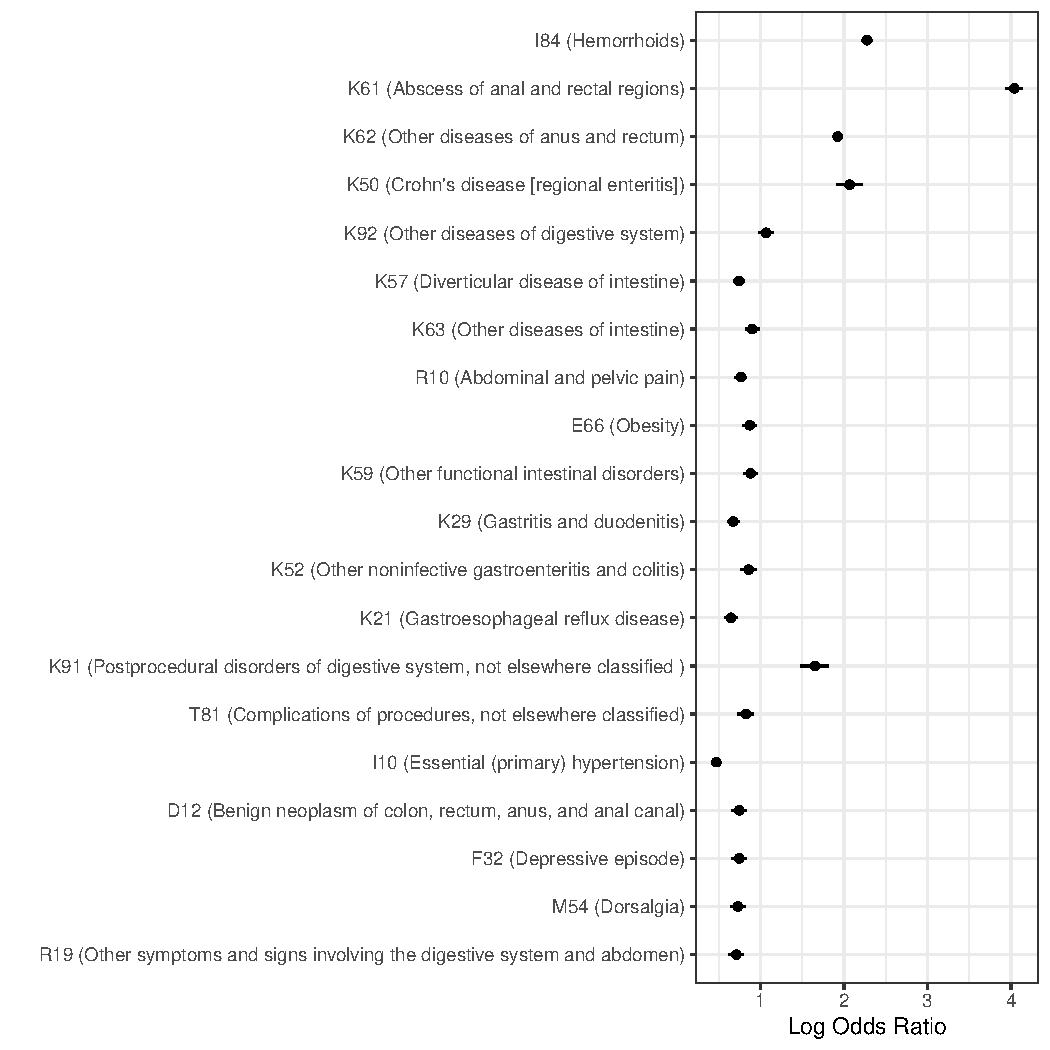
\includegraphics[width=1.0\textwidth]{pheno_enrich}
  \caption[Figure]{Top 20 ICD-10 codes enriched in pAD cases versus pAD controls ordered by Fisher's exact test P-value. Odds ratios and their 95\% confidence intervals were calculated using Fisher's exact test based on the number of pAD cases and controls with and without each particular ICD-10. Note that the control exclusion criteria in Table \ref{table:ukbb_ctrl_excl_criteria} were not applied in this analysis.}
  \label{fig:pheno_enrich}
  \end{figure}



  \subsection{Identifying genome-wide significant loci}
  Defining genome-wide significant loci in GWAS studies is often complicated by the widespread correlation between proximal genetic variants (i.e. linkage disequillibrium or LD). To identify pAD-associated loci, I used an LD clumping procedure, which outputs a set of \textit{index variants}, each representing a set of highly correlated variants in a locus. Additionally, LD clumping identifies nominally-associated variants that are highly correlated with the index variant at each locus (which I will refer to as LD friends; $R^{2}$ > 0.5 and P-value < 0.01; Methods). In total, seven independent loci achieved genome-wide significant association (P-value < $5\times10^{-8}$). All index variants were well-imputed (INFO $\geq$ 0.99). I also compared the index variants MAFs to population MAFs to ensure that they did not significantly deviate from expected MAFs in non-Finnish Europeans (NFE). All index variants' MAFs matched MAFs obtained from 1000 Genomes Project (1000GP; Table \ref{table:gws}; see Methods for how MAF deviation from the general population was formally assessed). 

  \begin{table}[htb]
    \centering\begingroup\fontsize{10}{14}\selectfont
    \caption{Genome-wide significant index variants in the UKBB analysis. Odds ratio and their 95\% confidence intervals are shown. Minor allele frequencies (MAF) in UKBB and 1000GP (NFE) are shown in the last two columns.}
    \label{table:gws}
    \begin{tabular}[t]{|l|l|l|l|l|l|l|}
      \hline
      Chromosome & Position (b38) & Effect Allele & Odds Ratio & P-value & MAF (UKBB) & MAF (1000GP)\\
      \hline
      3 & 52,992,368 & T & 1.13 (1.08 - 1.17) & $1.5\times10^{-8}$ & 0.42 & 0.44\\
      \hline
      6 & 31,044,486 & G & 1.13 (1.08 - 1.18) & $2.2\times10^{-8}$ & 0.37 & 0.37\\
      \hline
      6 & 31,113,288 & C & 1.13 (1.08 - 1.18) & $1.1\times10^{-8}$ & 0.41 & 0.44\\
      \hline
      6 & 31,113,923 & A & 1.12 (1.08 - 1.17) & $3.2\times10^{-8}$ & 0.49 & 0.49\\
      \hline
      6 & 31,148,469 & A & 1.12 (1.08 - 1.17) & $2.6\times10^{-8}$ & 0.44 & 0.45\\
      \hline
      9 & 22,119,196 & T & 0.89 (0.85 - 0.93) & $2.7\times10^{-8}$ & 0.48 & 0.47\\
      \hline
      11 & 10,356,352 & C & 0.88 (0.84 - 0.92) & $7.3\times10^{-9}$ & 0.29 & 0.30\\
      \hline
      \end{tabular}

    \endgroup{}

    \end{table}

    Four of the seven loci were located in the major histocompatibility complex region (MHC; 6p21.33), and one locus in each of 3p21.1, 9p21.3 and 11p15.4. The MHC region is known to be highly polymorphic and exhibits complex and long-range LD patterns, which complicate the definition of independent loci. 
    For example, two of the four MHC loci overlapped, with their two independent index variant located less than 700 bp apart. One of the two index variants (6:31113288\_T\_C) tagged a large number of variants ($R^{2}$ > 0.8) in the locus, while the other tagged no variants (6:31113923\_A\_G). Compared to the four MHC loci, the three non-MHC loci had less complex LD patterns. All three non-MHC index variants tagged a large number of variants and there was no overlapping independent loci in any of them. Given this complexity, I performed a number of post-GWAS checks to better understand the LD structure of all seven loci, which I will describe in the next section.


    \begin{figure}[H] 
      \centering    
      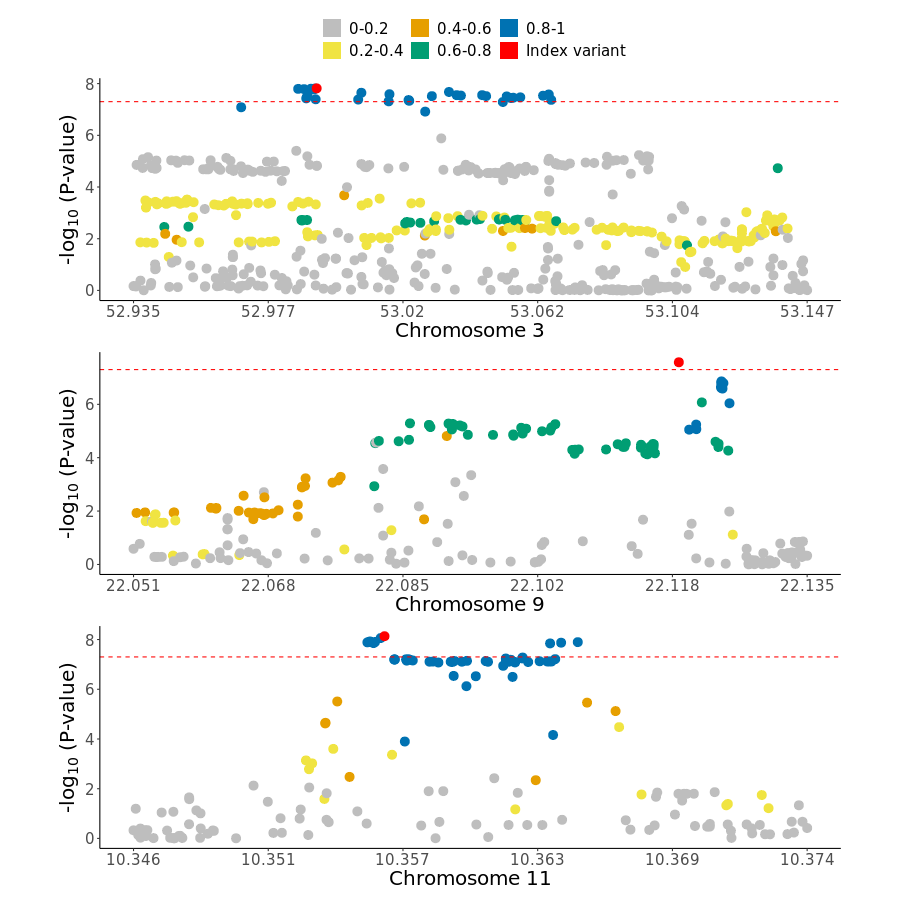
\includegraphics[width=1.0\textwidth]{Vector/ukbb_nonmhc_regional_assoc_plots.png}
      \caption[Figure]{Regional association plots for the three non-MHC loci, with position (build 38) plotted on the x-axis and $-log_{10}$ P-values shown on the y-axis for each variant. Colors indicate the $R^{2}$ between each variant and the index variant, and the red horizontal line indicates genome-wide significance (P-value = $5\times10^{-8}$).}
      \label{fig:ukbb_nonmhc_regional_assoc_plots}
      \end{figure}

      \begin{figure}[H] 
        \centering    
        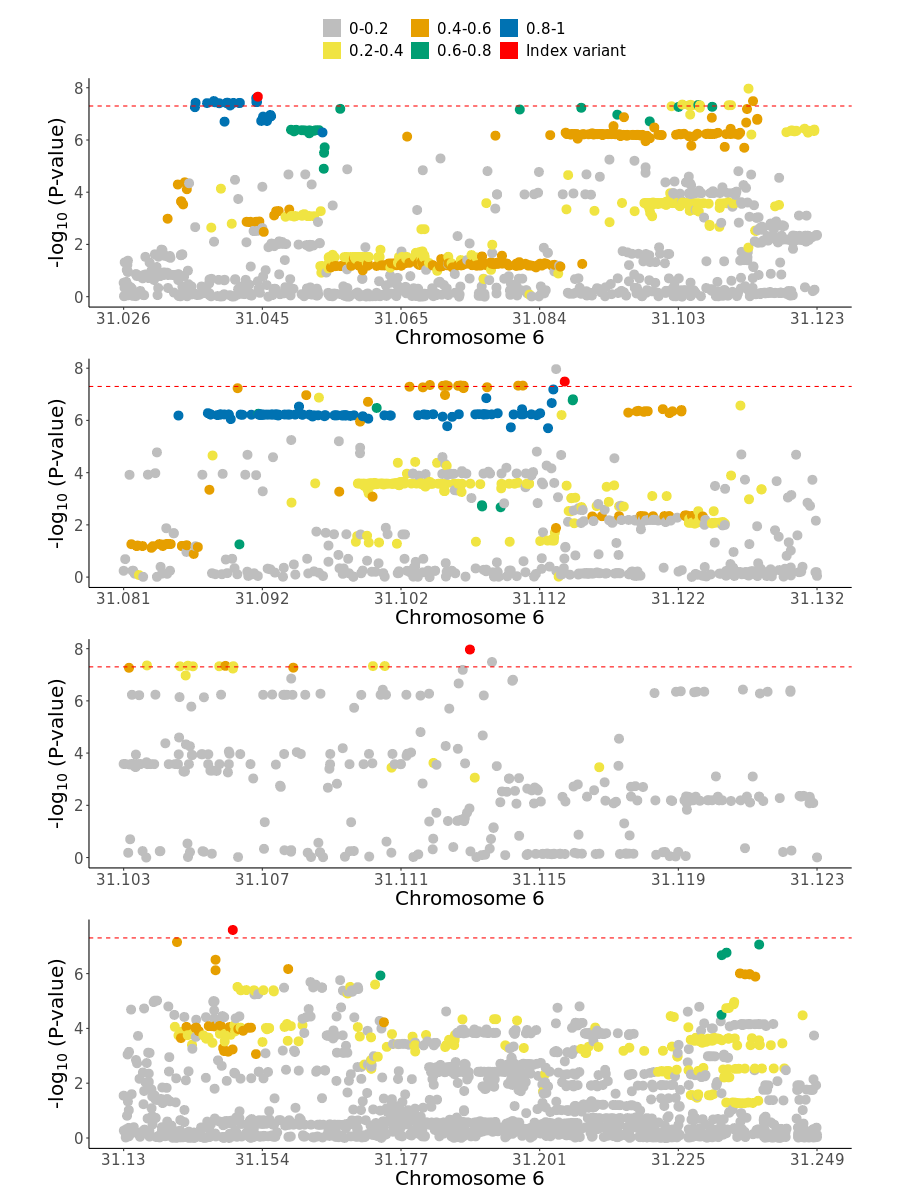
\includegraphics[width=1.0\textwidth]{Vector/ukbb_mhc_regional_assoc_plots.png}
        \caption[Figure]{Regional association plots for the four MHC loci, with position (build 38) plotted on the x-axis and $-log_{10}$ P-values shown on the y-axis for each variant. Colors indicate the $R^{2}$ between each variant and the index variant, and the red horizontal line indicates genome-wide significance (P-value = $5\times10^{-8}$). The second and third plots show the two overlapping MHC loci (index variants: 6:31113288\_T\_C and 6:31113923\_A\_G, respectively).}
        \label{fig:ukbb_mhc_regional_assoc_plots}
        \end{figure}

    \subsection{Post-GWAS quality checks}
    Spurious associations can seriously affect the validity of any significant results in GWAS studies. At the level of a single locus,  spurious associations can be diagnosed by assessing the relationship between the index variant and its LD friends. For a given variant in a genome-wide significant locus, the lower its LD with the index variant, the weaker its association is expected to be. Loci where the association strength of LD friends does not "decay" as expected given their LD with the index variant are therefore paricularly problematic. Specifically, such a mismatch would suggest that the LD strcuture that drives the observed association strength of LD friends does not match the general population LD. A possible source of this mismatch may be crpytic subpopulation stratification, which often contributes to false positive associations in GWAS \cite{Hellwege2017-xf}. \\ 
    
    I investigated the seven genome-wide significant loci to ensure the association signal follows the expected LD pattern in the general population. For this check to be valid, LD needs to be computed from a suitable matching reference panel such as 1000GP. Additionally, each index variant needs to have a number variants LD friends. To this end, I computed $R^{2}$ between each variant and the index variant at each locus using NFE individuals in 1000GP as a reference panel. For each pAD-associated locus, I quantified the correlation between $R^{2}$ and P-values (on the $-log_{10}$ scale) of each index variant's LD friends. Additionally, I performed two follow-up assessments for the loci where this correlation is weak ($\rho$ < 0.2) or cannot be computed due to a lack of LD friends. \\

    % \subsection{Index variants quality check}
    
    % All index variants were called in 1000GP except the index variant in 3p21.1 (3:52928665\_C\_T). Despite its high imputation quality in UKBB (INFO=0.93),  3:52928665\_C\_T was flagged as a low-quality site in gnomAD. Gnomad reports that 3:52928665 is a multi-allelic site located in a low-complexity region, and it is covered in fewer than 50\% of gnomAD's individuals. For this locus, I therefore computed LD with respect to the second most significant variant, which was also genome-wide significant (3:52992368\_C\_T; P-value=$1.5\times10^{-8}$). For the remaining three loci, I computed LD with the index variant for all variants in 1mbp window around the index variant. 
    
    \subsection{Relationship between P-value and LD} \label{sec:ukbb_postgwas}
  Index variants in 3p21.1, 9p21.3 and 11p15.4 had a large number of LD friends (N=63, 66, and 49, respectively), and the P-values for each index variants' LD friends were highly correlated with $R^{2}$ ($\rho$ = 0.98, 0.74, 0.83, respectively), indicating that the P-values closely match the expected LD pattern in
  NFE. Two of the MHC loci also showed a similar LD decay pattern (index variants 6:31044486\_G\_C and 6:31148469\_G\_A in Figure \ref{fig:ukbb_ld_decay_mhc}), with a strong correlation between P-values and $R^{2}$ (Figure \ref{fig:ukbb_ld_decay_mhc}). However, this correlation did not hold for the two other overlapping MHC loci mentioned earlier, which motivated me to further investigate these two loci (ndex variants: 6:31113288\_T\_C and 6:31113923\_A\_G).
  
  \subsubsection{A complex LD pattern at two MHC loci}
  \begin{figure}[H] 
    \centering    
    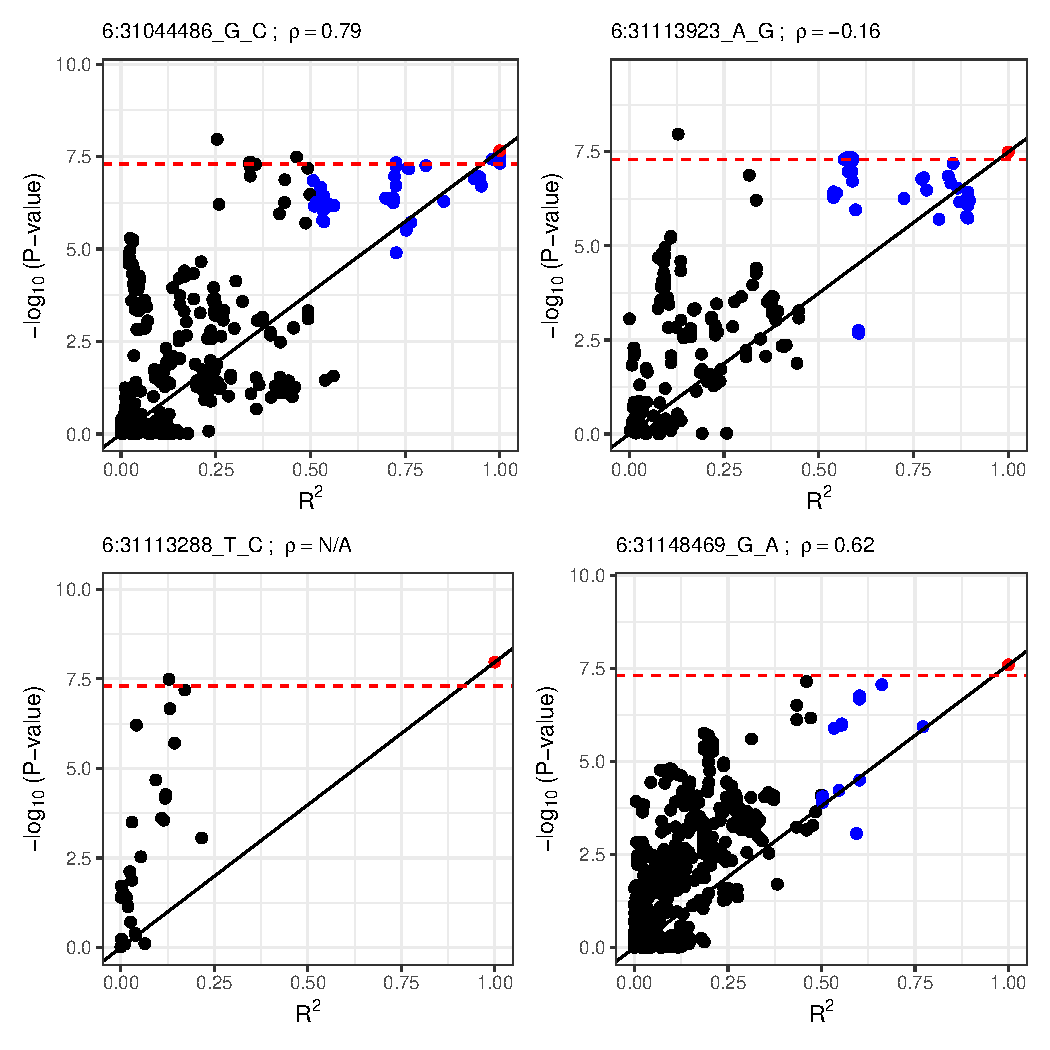
\includegraphics[width=0.8\textwidth]{ukbb_ld_decay_mhc}
    \caption[Figure]{LD decay plots showing association P-values for the four genome-wide significant loci in the MHC locus (x-axis) and each variant's $R^{2}$ with the index variant, derived from NFE in 1000GP (y-axis). Red dots and titles indicate the index variant in each locus. Blue dots indicate each index variant's LD friends, and the red horizontal line indicates genome-wide significance level (P-value < $5\times10^{-8}$). The black line is fitted to the origin (0,0), and to the point (1,$-log_{10}(P_{index\_variant})$), and shows the expected association strength given the LD with the index variant.}
    \label{fig:ukbb_ld_decay_mhc}
    \end{figure}
  First, one of MHC index variants at the two overlapping MHC loci did not tag any LD friends and therefore the correlation between P-value and $R^{2}$ could not be assessed (6:31113288\_T\_C in Figure \ref{fig:ukbb_ld_decay_mhc}). It is unclear whether the absence of LD friends for 6:31113288\_T\_C suggests that it is a truly indepent variant, or whether it is driven by a mismatch between the LD patterns in UKBB and 1000GP. Such a mismatch may lead to an underestimateion of LD between the index variant and its LD friends. To answer this question, I recalculated the LD values in 1000GP using only British individuals (GBR; N=90), and found that the index variant also did not tag any LD friends in 1000GP GBR as well. Given that 6:31113288\_T\_C is well-imputed (INFO=0.99) and common and that it is not well-tagged in both the NFE and GBR subpopulations in 1000GP, it is unlikely that the its association is driven by British-ancestry-specific LD. However, it is important to note that this does not rule out possible subpopulation stratification at this locus, which could potentially drive this association. 

  \begin{figure}[H] 
    \centering    
    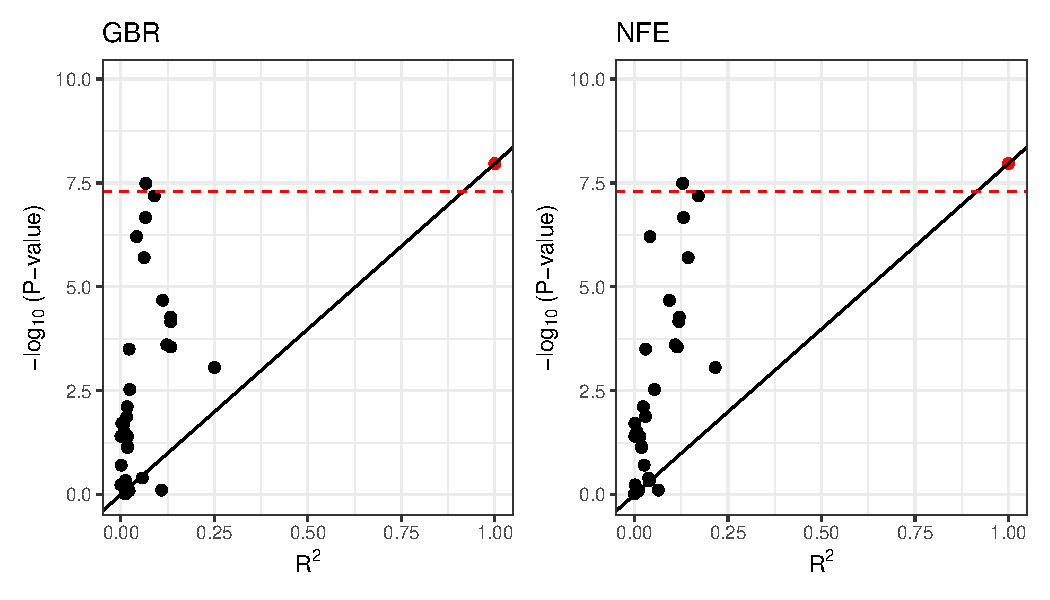
\includegraphics[width=0.8\textwidth]{ukbb_ld_decay_nfe_vs_gbr}
    \caption[Figure]{LD decay plots showing association P-values for the locus around index variant 6:31113288\_T\_C. Each variant's $R^{2}$ with the index variant, derived from NFE and GBR in 1000GP is shown on the x-axis and $-log_{10}$ P-values on the y-axis, showing that the index variant does not tag any LD friends in both NFE and GBR. Red dots indicate the index variant adn the red horizontal line indicates genome-wide significance level (P-value < $5\times10^{-8}$). The black line is fitted to the origin (0,0), and to the point (1,$-log_{10}(P_{index\_variant})$), and shows the expected association strength given the LD with the index variant.}
    \label{fig:ukbb_ld_decay_nfe_vs_gbr}
    \end{figure}

  Second, for the second overlapping locus, $R^{2}$ and P-values showed an inverse correlation (index variant 6:31113923\_A\_G in Figure \ref{fig:ukbb_ld_decay_mhc}; $\rho$=-0.16).  This inverse correlation between $R^{2}$ and P-values suggest that not all the LD friends' P-values conform to their expected P-values given their LD with the index variant. I hypothesised that the reversal of correlation may be caused by the subset of LD friends with $R^{2}$ close to the value used for defining LD friends. This subset could lead to an inverse correlation due to a stronger-than-expected P-value given their LD with the index variant. To this effect, I found that 10 LD friends had a genome-wide significant P-value (< $5\times10^{-8}$) despite all having an $R^{2}$ of 0.58 with the index variant. When I repeated the LD clumping procedure at this locus with a higher clumping $R^{2}$ cutoff (=0.6), I found that this subset of variants constituted a new genome-wide significant locus. This suggests that the identification of independent loci at this region is senstitive to the choice of LD clumping $R^{2}$ cutoff, which further complicates the identification of independent loci at this region. 
  

  



      \subsection{Finngen GWAS}
      Similar to UKBB, other national biobanks with genetic, clinical and phenotypic data are available. Although most national biobanks limit access to their individual-level genotype and phenotype data to approved researchers only, results from secondary analyses, including GWAS summary statistics, are made publicly available. \\

      FinnGen is a national biobank whose aim is to collect genetic and phenotypic data for 500,000 Finnish individuals. The latest data freeze (Data Freeze 9) has genotyped over 377,000 individuals and has carried out GWAS for over 2,200 clinical endpoints. FinnGen uses a different clinical coding system from ICD to organise phenotypes into endpoints (FinnGen endpoints). There are two main differences between UKBB and FinnGen in terms of their clinical code structure. First, most FinnGen endpoints have parallel ICD codes, but additional FinnGen endpoints are created at request. Bespoke endpoints define certain inclusion or exclusion criteria based on ICD codes, or sometimes combine codes from different ICD chapters to create a new endpoint. Second, FinnGen endpoints are curated by experts in each field and are constantly reviewed in different FinnGen data freezes. They are brodaly classified as \textit{core endpoints}, or \textit{non-core endpoints}. Basic statistics such as prevalence and gender ratios are calculated for all FinnGen endpoints, while GWAS is conducted only for core endpoints.\\

ICD-10 code K60 corresponds to FinnGen endpoint K11\_FISSANAL (Fissure and fistula of anal and rectal regions). K11\_FISSANAL defines cases and controls similar to my UKBB cohort definition outlined in Table \ref{table:ukbb_ctrl_excl_criteria}. However, K11\_FISSANAL was considered a core endpoint only until Data freeze 7, and GWAS summary statistics for K11\_FISSANAL are threfore unavailable in later data freezes. 

\subsection{Identification of genome-wide significant loci in Finngen}

In order to investigate if the seven UKBB genome-wide significant loci replicated in an independent cohort and to identify additional loci, I downloaded GWAS summary statistics for FinnGen's clinical endpoint K11\_FISSANAL. As of data freeze 7, Finngen reports 6,610 pAD cases and 253,186 controls. There was no further information regarding the subtypes of pAD (e.g. numbers of fissure and fistula cases), and it is therefore unclear if the composition of FinnGen's pAD case cohort is similar to the UKBB pAD case cohort. Understanding the differences in subphenotype composition of each cohort is important to understand if differences in association at genome-wide significant loci is driven by genetic factors (e.g. differences in MAFs or LD structure) or by phenotypic differences between the cohorts. 

After I filtered out variants with MAF < 0.01, a total of 9,054,355 variants remained. There was an acceptable level of genomic inflation (median $\chi^{2}$=0.495; $\lambda_{GC}$=1.089). To identify genome-wide significant loci, I used an LD clumping approach similar to the UKBB analysis, with the only difference being that I calculated LD from Finnish Europeans in 1000GP (FE; N=99). I found three genome-wide significant non-MHC loci: 1p34.2, 6p25.3 and 12q24.21 (P-value < $5\times10^{-8}$). Imputation quality information was not available in the downloaded summary statistics, so I was not able to confirm if the index variants had good imputation quality. However, the index variants' MAFs matched MAFs derived from FE in 1000GP, suggesting that they are imputed or genotyped with high accuracy (Table \ref{table:gws_finngen}). Furthermore, I performed similar post-GWAS checks to UKBB to ensure the P-value of the index variants LD friends match their expected values given their LD with the index variant. All three showed a good decay of P-values with LD ($\rho$=0.92, 0.74 and 0.44, respectively; Figure \ref{fig:finngen_regional_assoc_ld_decay_plots})

\begin{table}[htb]
  \centering\begingroup\fontsize{10}{12}\selectfont
  \caption{Genome-wide significant index variants in the FinnGen GWAS. Odds ratio and their 95\% confidence intervals are shown. Minor allele frequencies (MAF) in UKBB and 1000GP (FE) are shown in the last two columns.}
  \label{table:gws_finngen}
  \begin{tabular}[t]{|l|l|l|l|l|l|l|}
  \hline
  Chromosome & Position (b38) & Effect Allele & Odds Ratio & P-value & MAF (Finngen) & MAF (1000GP)\\
  \hline
  1 & 39,817,036 & T & 1.14 (1.09 - 1.19) & $7.2\times10^{-10}$ & 0.21 & 0.22\\
  \hline
  6 & 1,771,278 & T & 0.9 (0.87 - 0.93) & $6.7\times10^{-9}$ & 0.42 & 0.39\\
  \hline
  12 & 114,235,969 & T & 1.11 (1.07 - 1.15) & $7.0\times10^{-9}$ & 0.47 & 0.47\\
  \hline
  \end{tabular}
  \endgroup{}
  \end{table}

\begin{figure}[H] 
  \centering    
  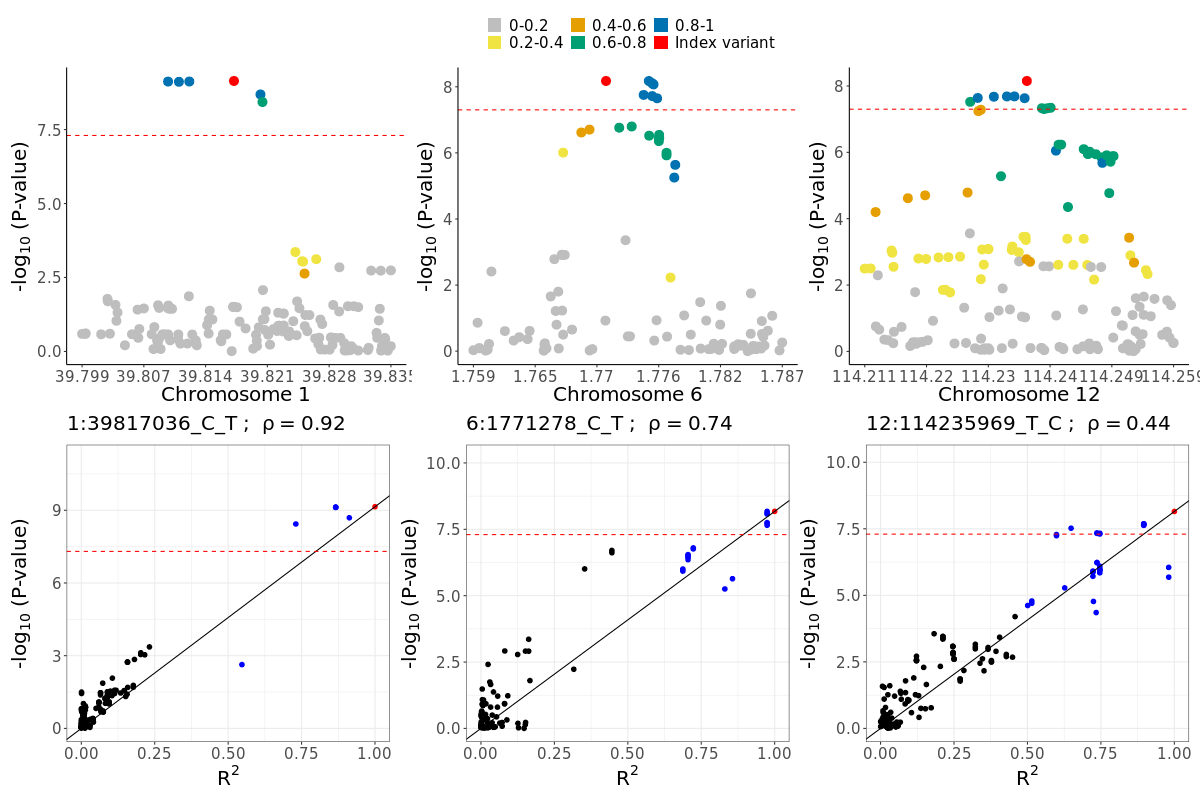
\includegraphics[width=1.0\textwidth]{Vector/finngen_regional_assoc_ld_decay_plots.png}
  \caption[Figure]{(Top) Regional association plots for the three FinnGen loci, with position plotted on the x-axis and $-log_{10}$ P-values shown on the y-axis for each variant. Colors indicate the LD value of each variant with the index variant, and the red horizontal line indicates genome-wide significance (P-value = $5\times10^{-8}$). (Bottom) LD decay plots showing association P-values for the three genome-wide significant loci in FinnGen (x-axis) and each variant's $R^{2}$ with the index variant, derived from FE in 1000GP (y-axis). Red dots and titles indicate the index variant in each locus. Blue dots indicate each index variant's LD friends. The red horizontal line indicates genome-wide significance level, and the black line is fitted to the origin (0,0), and to the point (1,$-log_{10}(P_{index\_variant})$), and shows the expected association strength given the LD with the index variant.}
  \label{fig:finngen_regional_assoc_ld_decay_plots}
  \end{figure}




\subsection{Replication of UKBB loci in Finngen}

\subsubsection{LD pattern in Finnish Europeans}
In GWAS studies, the true causal variant in an associated locus is often unknown due to LD between variants. Moreover, it is often the case that the true causal variant may not even be genotyped in array-based GWAS studies, or may not be imputed due to different imputation protocols and QC metrics being used in different GWAS. When assessing replication of a GWAS locus between two cohorts, it is therefore important to ensure that variants that are genotyped or imputed in the two cohorts have similar LD structures. Indeed, a lack of GWAS hit replication is sometimes driven by a difference in LD patterns between the two studies under comparison, one of which may not have genotyped or imputed any variants that tag the true causal variant in its respective population \cite{Kraft2009-xg}. Finnish Europeans (FE) and NFE are known to exhibit systematic difference in their LD strucure, which may affect the ability to replicate the pAD-associated loci discovered in the UKBB. To compare the LD pattern between FE and NFE at the pAD-associated loci, I computed the LD between each variant and the index variant in the FE and NFE subpopulations of 1000GP.\\





% \begin{figure}[H] 
%   \centering    
%   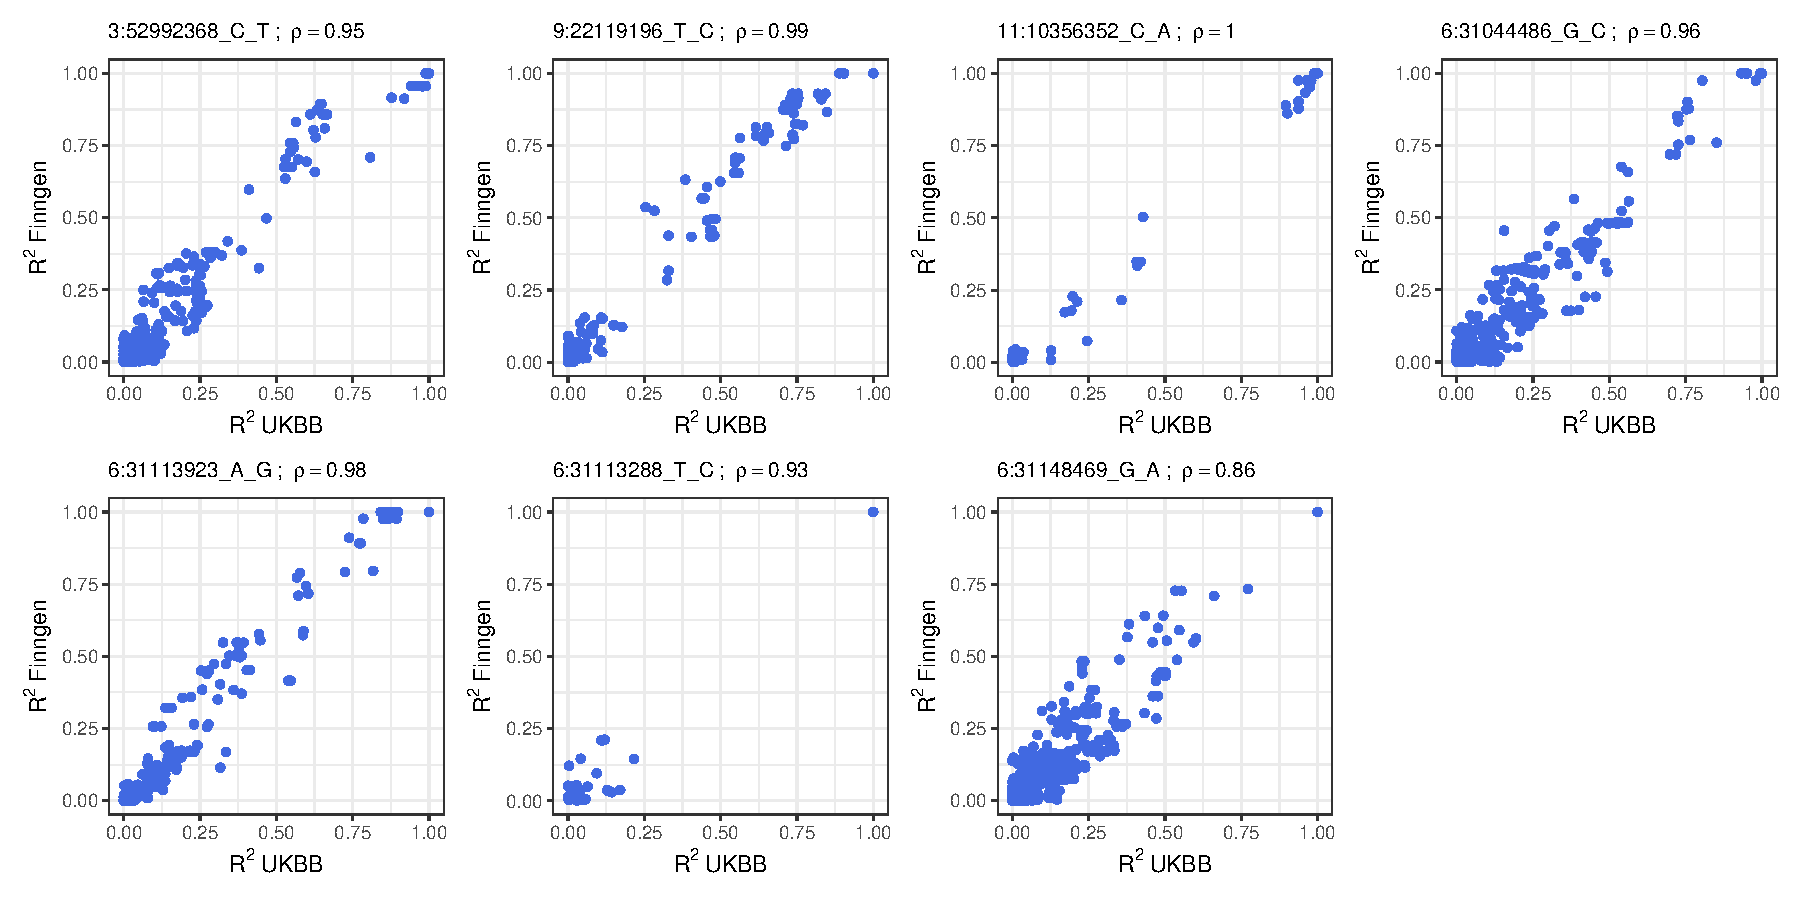
\includegraphics[width=1.0\textwidth]{ukbb_finngen_ld_plot}
%   \caption[Figure]{$R^{2}$ between variants and the index variant in the four pAD-associated loci in non-Finnish Europeans (x-axis) and Finnish Europeans (y-axis). $R^{2}$ values are derived from the 1000GP. Pearson correlation coefficients and index variants are indicated on top of each figure.}
%   \label{fig:ukbb_finngen_ld_plot}
%   \end{figure}
\captionsetup[subfigure]{font={normal,small}, skip=1pt, margin=-0.7cm, singlelinecheck=false,position=top}
	

\begin{figure}[H]
  \centering
  \begin{subfigure}[b]{1.0\textwidth}
      \centering
      \caption{}
      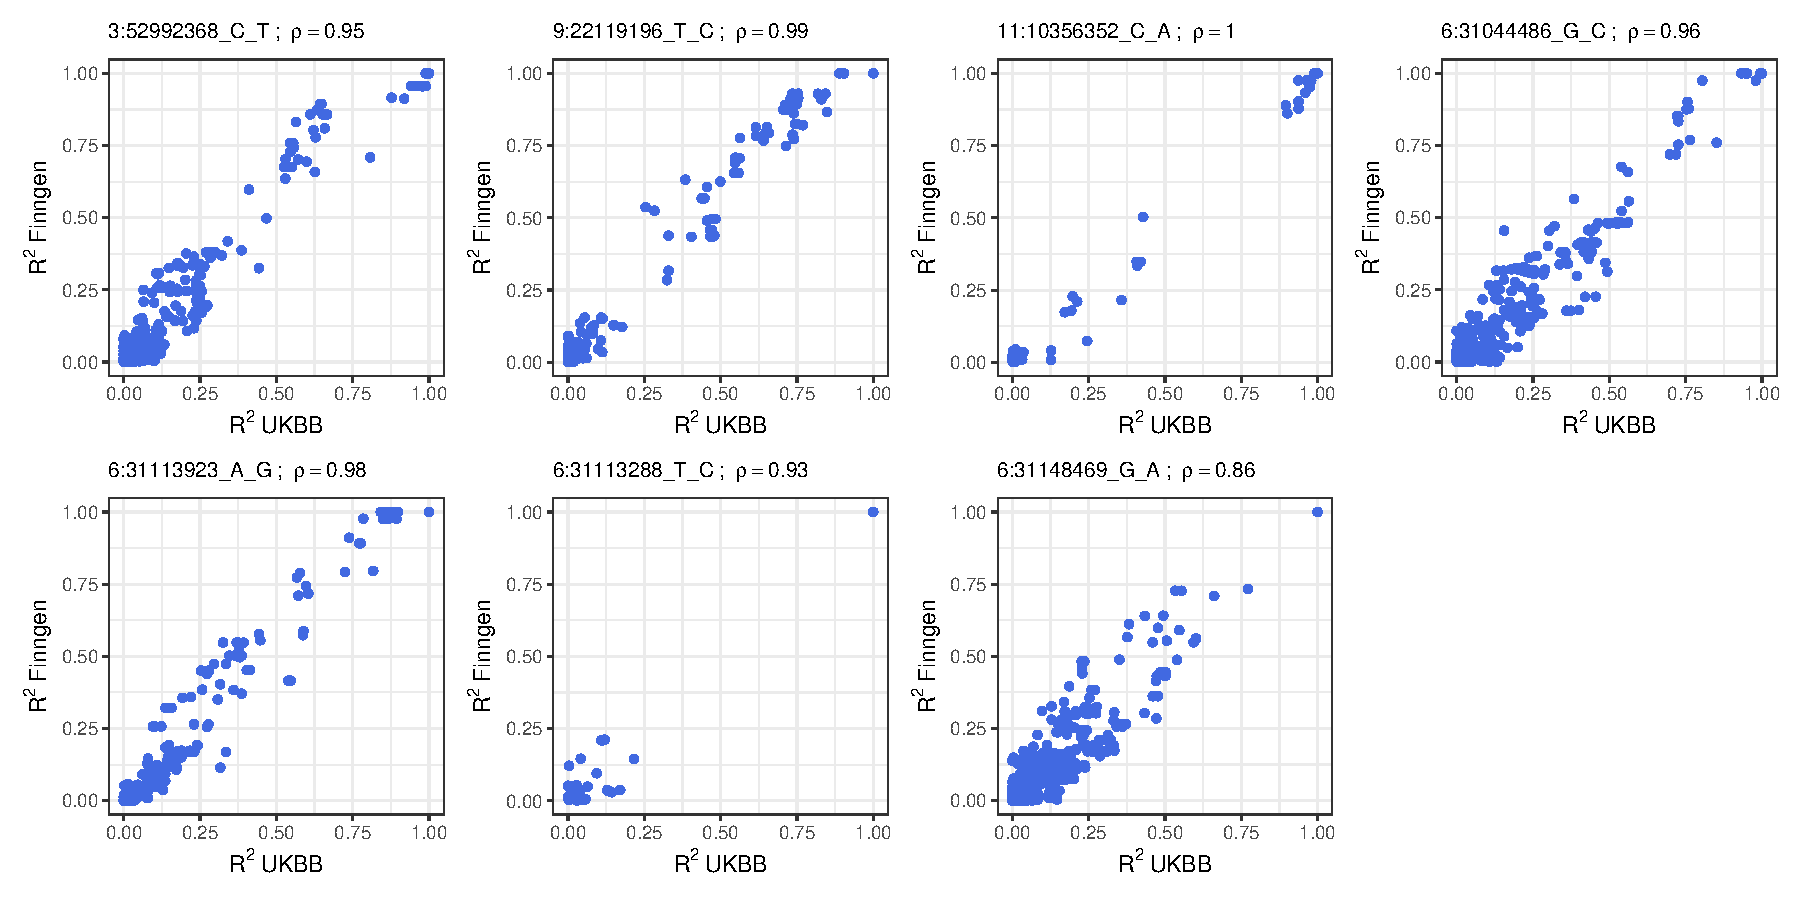
\includegraphics[width=\textwidth]{ukbb_finngen_ld_plot}
      
      \label{fig:ukbb_finngen_ld_plot}
  \end{subfigure}
  \hfill
  \begin{subfigure}[b]{1.0\textwidth}
      \centering
      \caption{}
      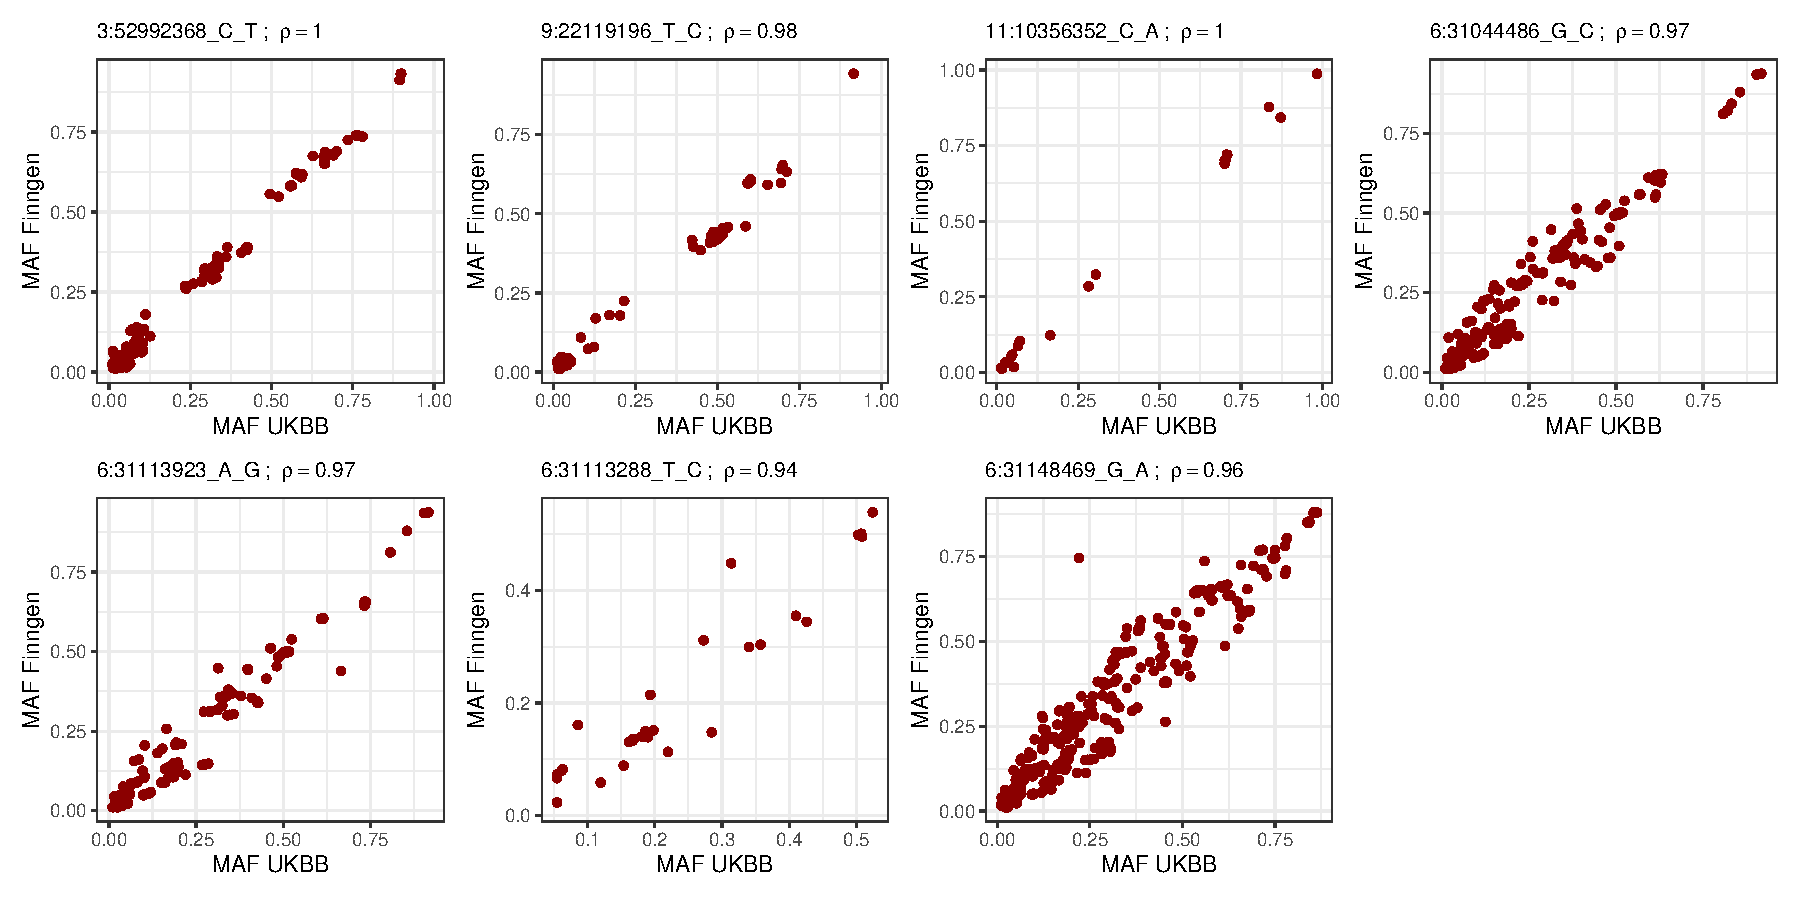
\includegraphics[width=\textwidth]{ukbb_finngen_maf_plot}
      
      \label{fig:ukbb_finngen_maf_plot}
  \end{subfigure}


     \caption{(a) $R^{2}$ between all variants within each locus' boundaries and the index variant in the seven genome-wide significant loci identified in UKBB. $R^{2}$ are derived from non-Finnish Europeans (x-axis) and Finnish Europeans (y-axis) in 1000GP. Pearson correlation coefficients and index variants are indicated on top of each figure. (b) MAF of all variants in the UKBB (x-axis) and FinnGen (y-axis).}
     \label{fig:ld_maf_replication_ukbb_in_finngen}
\end{figure}
I found that MAF was nearly perfectly correlated in NFE and FE in all seven pAD-associated loci ($\rho$ > 0.94; Figure \ref{fig:ld_maf_replication_ukbb_in_finngen}a). $R^{2}$ were also strongly correlated in all loci ($\rho$ > 0.86; Figure \ref{fig:ld_maf_replication_ukbb_in_finngen}b). Notably, despite a strong $R^{2}$ correlation, 6:31113288\_T\_C did not have any LD friends in FE, similar to GBR and NFE, and the strong correlation at this locus was driven by variants with a low $R^{2}$ with the index variant. Overall, witht the exception of 6:31113288\_T\_C which did not have any LD friends in FE, both MAF and the LD structure were consistent across all pAD-associated loci between NFE and FE. Replication of UKBB hits can therefore be reasonably assessed in the FinnGen GWAS. I found that two UKBB non-MHC index variants replicated in FinnGen (FinnGen P-value < $7\times10^{-3}$ for 7 variants; Table \ref{table:replication_ukbb_in_finngen}), and that neither of them showed evidence of heterogeneity fo effect size ($P_{het}$ < $7\times10^{-3}$; Table \ref{table:replication_ukbb_in_finngen}). Additionally, all the five index variants that failed to replicate also showed evidence of heterogeneity of effect sizes.

% \subsubsection{UKBB non-MHC loci replicate in Finngen}
% To test the replication of the UKBB hits, I adopted an approach that takes into account subtle differences in LD between FE and NFE. UKBB index variants may not necessarily tag the true causal variants in FE, and an absence of replication of the exact UKBB index variants in FinnGen does not therefore indicate the lack of association at pAD-associated loci. Therefore, I performed the replication using each index variant and their LD friends in FinnGen ($R^{2}$ > 0.5 in FE). 

\begin{table}[H]
  \centering\begingroup\fontsize{10}{12}\selectfont
  
  \caption{Replication of the UKBB genome-wide significant index variants in FinnGen. Odds ratio and their 95\% cofidence intervals are shown for both cohorts. The heterogeneity of effect P-value is shown in the last column. Only two index variants passed the replication threshold (3:52992368\_C\_T  and 11:10356352\_C\_A)}
  \label{table:replication_ukbb_in_finngen}
  \begin{tabular}[t]{llllll}
  \toprule
  Index variant & P-value UKBB & FinnGen P-value & OR UKBB & OR FinnGen & $P_{het}$\\
  \midrule
  3:52992368\_C\_T & $1.5\times10^{-08}$ & $1.2\times10^{-03}$ & 1.13 (1.08 - 1.17) & 1.06 (1.02 - 1.1) & $0.03$\\
  6:31044486\_G\_C & $2.2\times10^{-08}$ & $5.7\times10^{-02}$ & 1.13 (1.08 - 1.18) & 1.04 (1 - 1.07) & $1.9\times10^{-03}$\\
  6:31113923\_A\_G & $3.2\times10^{-08}$ & $3.9\times10^{-02}$ & 1.12 (1.08 - 1.17) & 1.04 (1 - 1.07) & $3.6\times10^{-03}$\\
  6:31113288\_T\_C & $1.1\times10^{-08}$ & $1.5\times10^{-01}$ & 1.13 (1.08 - 1.18) & 1.03 (0.99 - 1.07) & $7.2\times10^{-04}$\\
  6:31148469\_G\_A & $2.6\times10^{-08}$ & $9.9\times10^{-01}$ & 1.12 (1.08 - 1.17) & 1 (0.97 - 1.04) & $2.0\times10^{-05}$\\
  9:22119196\_T\_C & $2.7\times10^{-08}$ & $2.0\times10^{-02}$ & 0.89 (0.85 - 0.93) & 0.96 (0.93 - 0.99) & $6.0\times10^{-03}$\\
  11:10356352\_C\_A & $7.3\times10^{-09}$ & $3.4\times10^{-07}$ & 0.88 (0.84 - 0.92) & 0.91 (0.87 - 0.94) & $0.27$\\
  \bottomrule
  \end{tabular}
  \endgroup{}
  \end{table}




  \subsection{Replication of FinnGen loci in UKBB}
  Following the same replication approach, I tested the replication of FinnGen's three genome-wide significant loci in the UKBB GWAS. I found evidence of replication for all three index variants in the UKBB (UKBB P-value < 0.017 for 3 variants), and none of the variants showed evidence of heterogeneity of effect sizes ($P_{het}$ < 0.017; Table \ref{table:replication_finngen_in_ukbb}).

  \begin{table}[H]
    \centering\begingroup\fontsize{10}{12}\selectfont
    \caption{Replication of the FinnGen genome-wide significant index variants in UKBB. Odds ratio and their 95\% cofidence intervals are shown for both cohorts. The heterogeneity of effect P-value is shown in the last column.}
    \label{table:replication_finngen_in_ukbb}
    \begin{tabular}[t]{llllll}
    \toprule
    Index variant & P-value UKBB & FinnGen P-value & OR UKBB & OR FinnGen & $P_{het}$\\
    \midrule
    1:39817036\_C\_T & $1.6\times10^{-06}$ & $7.2\times10^{-10}$ & 1.13 (1.08 - 1.19) & 1.14 (1.09 - 1.19) & $0.77$\\
    6:1771278\_C\_T & $1.5\times10^{-04}$ & $6.7\times10^{-09}$ & 0.91 (0.87 - 0.96) & 0.9 (0.87 - 0.93) & $0.63$\\
    12:114235969\_T\_C & $1.3\times10^{-03}$ & $7.0\times10^{-09}$ & 1.07 (1.03 - 1.12) & 1.11 (1.07 - 1.15) & $0.2$\\
    \bottomrule
    \end{tabular}
    \endgroup{}
    \end{table}


    \subsection{Meta-analysis of UKBB and FinnGen}
    Meta-analysis between GWAS cohorts is commonly used to increase statistical power to identify genome-wide significant loci. Practically, meta-analysis is carried out when the are constraints on sharing individual-level data, or when genotype data from several studies cannot be combined \cite{Evangelou2013-rn}. In these cases, meta-analysis of association summary statistics is the preferred analytical approach, and there is ample evidence that it achieves similar statistical power as combining genotype data from several studies \cite{metal_docs}. \\



    \subsubsection{Meta-analysis and identification of genome-wide significant loci}
    I performed a fixed-effects meta-analysis between UKBB and FinnGen effect sizes and standard errors using METAL (see Methods for more details). Because I performed a meta-analysis between two GWAS summary statistics from Finnish and Non-Finnish Europeans, I performed LD clumping separately with an LD panel from each of the two populations, and found 18 genome-wide significant loci (P-value < $5\times10^{-8}$). I tested whether the index variants' effect size estimates were consistent between UKBB and FinnGen using Cochran's Q test, which is implemented in METAL (Methods). A strong deviation from the null hypothesis that effect sizes are similar between UKBB and FinnGen reflects uncertainty around the meta-analysed effect size estimate. To this end, I found no evidence of heterogenity for any of the 12 index variants ($P_{het} < 4\times10^{-3}$). Furthermore, I compared the association signal and LD for each locus using same two reference panels. Six of these loci either showed weak or inverse correlation between P-values and $R^{2}$ derived from either NFE and FE ($\rho$ < 0.2), and were therefore removed from the rest of the downstream analyses (more details in Methods).\\
    
    % Furthermore, for the remaining 12 genome-wide significant loci, 

    \begin{table}[H]

      \caption{\label{tab:table:meta_gws}Meta-analysis genome-wide significant loci (P-value < $5\times10^{-8}$), showing the index variant at each locus, the meta-analysis P-value, and the odds ratio in the UKBB, FinnGen, and meta-analysis. 95\% confidence intervals are shown for each odds ratio value. The last column shows the P-value of the effect size heterogeneity test, where $P_{het} < 4\times10^{-3}$ suggests evidence of heterogeneity of effects. The six loci that failed the LD decay test are highlighted in bold.}
      \centering
      \fontsize{10}{12}\selectfont
      \begin{tabular}[t]{llllll}
      \toprule
      Index variant & \makecell{Meta-analysis\\ P-value} & \makecell{OR\\ UKBB} & \makecell{OR\\ FinnGen} & \makecell{OR\\ Meta-analysis} & $P_{het}$\\
      \midrule
      \textbf{1:39809417\_A\_T} & $7.4\times10^{-15}$ & 1.13 (1.08 - 1.19) & 1.14 (1.09 - 1.19) & 1.14 (1.1 - 1.17) & 0.84\\
      \addlinespace
      \textbf{1:39836225\_G\_C} & $4.1\times10^{-08}$ & 1.09 (1.04 - 1.15) & 1.11 (1.06 - 1.16) & 1.1 (1.07 - 1.14) & 0.63\\
      \addlinespace
      3:53034026\_C\_T & $7.5\times10^{-10}$ & 1.13 (1.08 - 1.17) & 1.07 (1.03 - 1.11) & 1.09 (1.06 - 1.12) & 0.05\\
      \addlinespace
      5:64868326\_TTTC\_T & $2.0\times10^{-08}$ & 0.89 (0.85 - 0.93) & 0.94 (0.91 - 0.98) & 0.92 (0.89 - 0.95) & 0.05\\
      \addlinespace
      6:1775202\_G\_A & $1.0\times10^{-11}$ & 0.91 (0.87 - 0.95) & 0.9 (0.87 - 0.93) & 0.9 (0.88 - 0.93) & 0.80\\
      \addlinespace
      6:31121854\_C\_T & $4.2\times10^{-08}$ & 1.11 (1.07 - 1.16) & 1.06 (1.02 - 1.1) & 1.08 (1.05 - 1.11) & 0.08\\
      \addlinespace
      6:31253340\_T\_C & $3.8\times10^{-08}$ & 1.1 (1.06 - 1.15) & 1.07 (1.03 - 1.1) & 1.08 (1.05 - 1.11) & 0.24\\
      \addlinespace
      \textbf{6:133008360\_T\_A} & $2.7\times10^{-08}$ & 1.12 (1.07 - 1.19) & 1.1 (1.05 - 1.15) & 1.11 (1.07 - 1.15) & 0.47\\
      \addlinespace
      6:133260944\_G\_A & $4.7\times10^{-08}$ & 1.11 (1.06 - 1.17) & 1.08 (1.04 - 1.13) & 1.1 (1.06 - 1.13) & 0.42\\
      \addlinespace
      \textbf{6:133267939\_T\_C} & $4.5\times10^{-08}$ & 1.09 (1.05 - 1.14) & 1.07 (1.03 - 1.11) & 1.08 (1.05 - 1.11) & 0.42\\
      \addlinespace
      7:2524404\_G\_A & $4.1\times10^{-08}$ & 1.14 (1.07 - 1.22) & 1.13 (1.06 - 1.2) & 1.14 (1.09 - 1.19) & 0.76\\
      \addlinespace
      8:70735125\_A\_G & $3.9\times10^{-11}$ & 0.83 (0.77 - 0.9) & 0.82 (0.76 - 0.89) & 0.83 (0.78 - 0.87) & 0.94\\
      \addlinespace
      8:70993166\_AAGTT\_A & $1.2\times10^{-10}$ & 0.83 (0.77 - 0.9) & 0.82 (0.75 - 0.88) & 0.82 (0.78 - 0.87) & 0.75\\
      \addlinespace
      \textbf{9:21995045\_T\_G} & $4.3\times10^{-08}$ & 1.41 (1.25 - 1.59) & NA & 1.41 (1.25 - 1.6) & 1.00\\
      \addlinespace
      9:22124505\_A\_T & $2.1\times10^{-08}$ & 0.9 (0.86 - 0.93) & 0.95 (0.91 - 0.98) & 0.92 (0.9 - 0.95) & 0.05\\
      \addlinespace
      \textbf{10:61661180\_A\_G} & $2.0\times10^{-08}$ & 1.09 (1.04 - 1.14) & 1.08 (1.05 - 1.12) & 1.09 (1.06 - 1.12) & 0.90\\
      \addlinespace
      11:10356352\_C\_A & $1.3\times10^{-13}$ & 0.88 (0.84 - 0.92) & 0.91 (0.87 - 0.94) & 0.89 (0.87 - 0.92) & 0.27\\
      \addlinespace
      12:114235969\_T\_C & $4.2\times10^{-10}$ & 1.07 (1.03 - 1.12) & 1.11 (1.07 - 1.15) & 1.09 (1.06 - 1.12) & 0.20\\
      \bottomrule
      \end{tabular}
      \end{table}
      

  %   Why performed meta-analysis? 
  %   \begin{itemize}
      
      
  %     \item \textbf{Pros} 
  %     \item Any concerns about difference in phenotype definitions: 
  %     \item reasons why that might be the case (difference in proporion - biases introduced by different clinical systems - differences in prevalence)
  %     \item Any concerns about differences in LD and MAF and subpopulation stratification and how that was adressed
  %     \item \textbf{Cons}
  %     \item  Maximise in power
  %     \item pop strat can be taken care of by adjusting lambda gc
  %     \item Individual-level data are required for better definition of phenotype
  % \end{itemize}
    
 

  \subsection{Disentangling the genetic effect of pAD-associated variants on haemorrhoids}

  In section \ref{section:pheno_enrich}, I analysed the composition of the pAD case cohort and showed that it is significantly enriched with 198 ICD-10 clinical codes compared to pAD controls. Haemorrhoids was the most strongly eniched phenotype in pAD cases versus controls. I hypothesised that this enrichment was also reflected at the level of genetic risk predisposition. To confirm this, I carried out a genetic correlation analysis between the pAD meta-analysis and the Pan-UKBB haemorrhoids GWAS. I found strong evidence of high genetic correlation (ICD-10 code I84; P-value=$5.37\times10^{-26}$; $r_{g}$=0.66). To validate this correlation, I repeated the genetic correlation analysis using a larger haemorrhoids GWAS of over 900,000 individuals by Zheng et al. 2021 \cite{Zheng2021-ss}. I found a similar genetic correlation estimate that was even more significant than the estimate from the Pan-UKBB analysis ($r_{g}$=0.63; P-value=$10^{-62}$).\\
  

  The existence of a strong genetic correlation and enrichment of haemorrhoids could be explained by several factors. First, pAD could be a co-morbidity of haemorrhoids, in a similar way that Type 2 diabetes and obesity are co-morbidities. This could be a result of the same risk factors (genetic or otherwise) underlying both diseases, potentially with varying effect sizes. Alternatively, clinical diagnostic factors could also account for this overlap. Both diseases are among the differential diagnoses for patients presenting with rectal pain, swelling, bleeding and discharge. Therefore, a patient suffering from inflammed haemorrhoids is more likely to be diagnosed if they also suffer from pAD (e.g. after performing rectal examination). \\ 

Bias introduced by clinical diagnostic factors cannot be completely addressed with observational data, as this will require constructing pAD case-control cohorts where haemorrhoids cases are  balanced in both cases and controls. However, the impact of such bias could also be assessed by performing a pAD GWAS where haemorrhoids cases are excluded from cases and controls (pADexclHaem), and a haemorrhoids GWAS where pAD cases are excluded from cases and controls (HaemexclpAD). Comparing the genetic association effect sizes of the previously reported 12 index variants between pADexclHaem and HaemexclpAD may give an indication as to which genetic variants are likely to underlie both diseases and which are likely to be specific to pAD. \\

Constructing the two cohorts requires access to a individual-level phenotypic data in both UKBB and FinnGen. Since I do not have access to FinnGen's phenotype data, I tested the hypothesis that effect sizes are different between haemorrhoids and pAD in the UKBB only. To construct the HaemexclpAD case and control cohorts, I selected individuals who have been diagnosed with ICD-10 code I84 or ICD-9 code 455 in at least one inpatient episode as cases and excluded individuals with ICD-10 code K60 or ICD-9 code 565 from both cases and controls. Similarly, for pADexclHaem, I selected individuals who have been diagnosed with ICD-10 code K60 or ICD-9 code 565 in at least one inpatient episode and excluded individuals with ICD-10 code I84 or ICD-9 code 455 from both cases and controls. Additionally, I applied the same control exclusion criteria in Table \ref{table:ukbb_ctrl_excl_criteria}. 

\begin{figure}[H]
  \centering    
  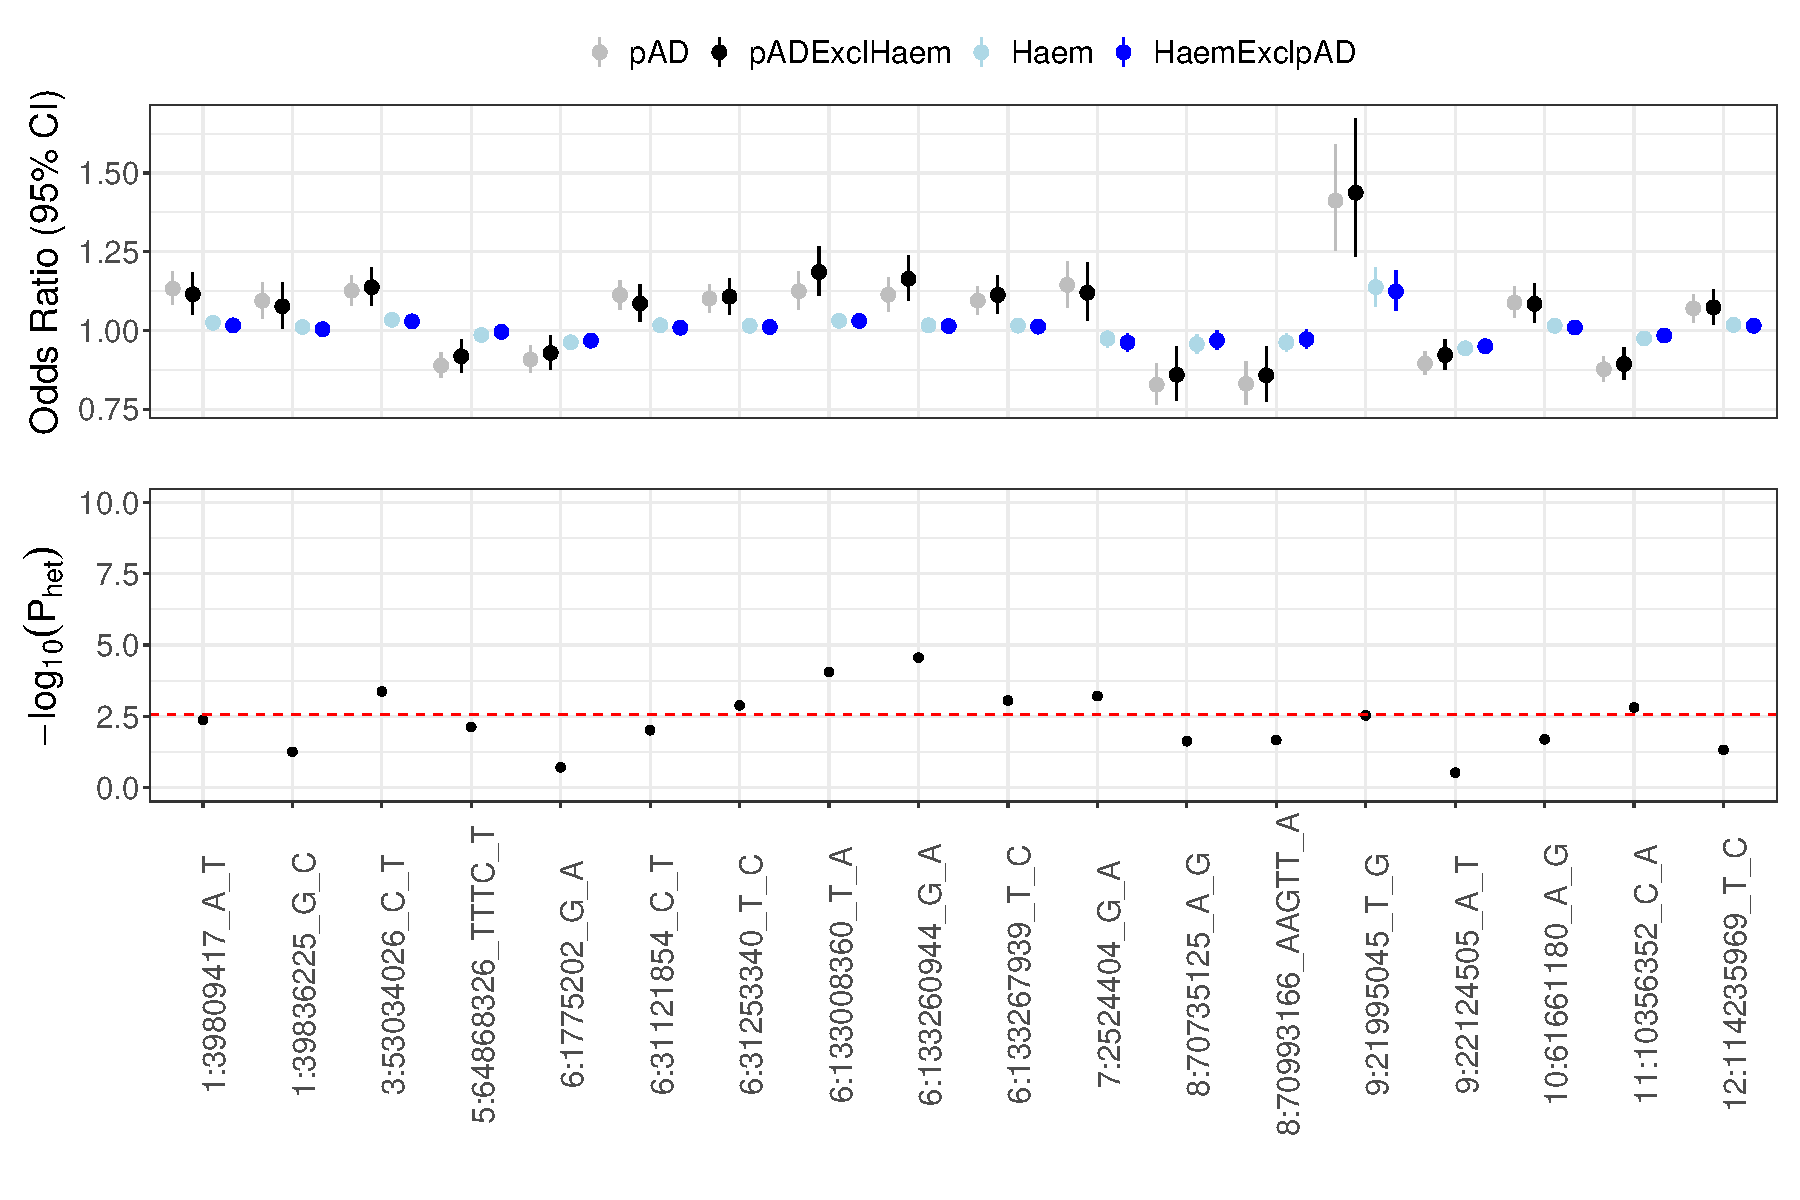
\includegraphics[width=1.0\textwidth]{combined_forest_het_plt}
  \caption[Figure]{Top plot shows the ffect sizes of the 12 pAD-assocaited index variants from four UKBB case/control cohorts: pAD in grey ($N_{case}$=4,606), pADExclHaem in black ($N_{case}$=2,799), Haem in light blue ($N_{case}$=29,285), and HaemExclpAD in blue ($N_{case}$=27,477). Bottom plot shows the heterogeneity of effect-size P-value ($P_{het}$) between the two disjoint GWAS analyses: pADExclHaem and HaemexclpAD. The red dotted line shows $P_{het}$ significance threshold ($P_{het} < 4\times10^{-3}$).}
  \label{fig:combined_forest_het_plot}
  \end{figure}

I tested the association of each of the 12 pAD-associated index variants with each of the four phenotypes described above. First, I examined if any of the index variants were associated with the two haemorrhoids phenotypes Haem and HaemExclpAD. Since I performed a targeted association test, I set a more permissive assocition threshold for declaring significance than normally used to declare genome-wide assoctions (P-value < $4\times10^{-3}$ for 12 variants). Despite the large difference in statistical power between the two haemorrhoids cohorts and the two pAD cohorts, I found that only three of the tested index variants achieved significant association in the better-powered haemorrhoids GWASes (index variants: 3:53034026\_C\_T, 6:1775202\_G\_A, and 9:22124505\_A\_T). Additionally, all three variants were significant in both Haem and HaemExclpAD, suggesting that the exclusion of pAD cases from the haemorrhoids cohort has little impact on their association. Moreover, 3:53034026\_C\_T showed significant evidence of effect size heterogeneity between pADExclHaem and HaemExclpAD ($P_{het}$ < $3\times10^{-3}$; Figure \ref{fig:combined_forest_het_plot}), with a significantly larger effect on pADExclHaem ($OR_{pADExclHaem}=1.14-1.2$ and $OR_{HaemExclpAD}=1.03-1.05$).\\

Although the other 11 index variants did not show a significant association with the two haemorrhoids definitions, four of them had significantly smaller effect sizes in HaemexclpAD than in pADexclHaem ($P_{het}$ < $4\times10^{-3}$; Figure \ref{fig:combined_forest_het_plot}). Moreover, five additional variants had suggestive evidence of heterogeneity of effect ($P_{het}$ < 0.05), and for all five variants the effect size was larger in pADExclHaem than in HaemExclpAD. \\

Two conclusion can be made from this analysis. First, despite a much larger sample size in favour of the haemorrhoids cohorts, only three pAD-associated index variants were also associated with haemorrhoids, even with a relatively lenient threshold for association. Second, despite their nominal association with haemorrhoids, these three variants (and indeed all other variants) had a consistently smaller effect size on HaemExclpAD than pADExclHaem, and for 3:53034026\_C\_T that difference in effect size was significant. More importantly, this pattern was observed for all 12 index variants, despite the lack of power to detect a significant heterogeneity of effects. Performing a similar 'disentaglment' analysis in both FinnGen and UKBB, and subsequently identifying which variants have a significantly larger effect size in pADExclHaem than HaemExclpAD is a plausible way to validate this pattern. Such validation would more strongly establish these variants as bona fidae pAD-associated variants, with a significantly smaller effect size on haemorrhoids.\\



\subsection{Identification of effector genes via colocalisation analysis} \label{sec:coloc}
Many GWAS loci that have been uncovered over the last 15 years are located in non-coding regions. This complicates the task of understanding their downstream effects and linking them to effector genes. Over the last ten years, large-scale studies that map genetic variants associated with transcriptomic variation have improved our understanding of the downstream effects of disease-associated genetic variants. For example, the Gentype Expression Project (GTEx) has mapped genetic variants associated with individual variation in overall levels of gene expression (eQTL) and splicing (sQTL). Additionally, statistical methods that are able to integrate association signals from different studies have been applied to GWAS and QTL data in order to investigate which effector genes likely underpin disease-associated GWAS signals. Colocalisation analysis, for example, quantifies the probability that two association signals are driven by a single causal variant ($PP_{4}$) and can therefore be used to compare GWAS and QTL association signals (more details in the Methods section).\\

I carried out colocalisation analysis between the 12 pAD-associated loci and eQTL and sQTL signals from GTEx v8 in a 1 mbp window centered around each locus' index variant. Across all 49 GTEx tissues, I performed the colocalisation with a total of 293 genes and all their splice junctions (see Methods for the number of genes and splice junctions tested at each locus).\\

The most informative output of colocalisation analysis is $PP_{4}$, the posterior probability of two association signals sharing a single underlying variant. Overall, I found high-confidence colocalisation evidence for seven loci, where at least one eQTL or sQTL colocalised with the association signal ($PP_{4}$ > 0.8; Table \ref{table:coloc_res}). All seven loci had at least a single colocalisation with an sQTL (12 sQTL genes), while five loci colocalised with at least one eQTL signal (eight eQTL genes), implicating a total of 15 genes. At many loci where both an eQTL and sQTL colocalisation were detected, distinct eQTL and sQTL genes were implicated. Moreover, QTLs in different tissues often implicated different genes. For example, the locus at index variant 7:2524404\_G\_A colocalised with two different genes (\textit{BRAT1} in the liver and thyroid gland, and \textit{LFNG} in the skin and whole blood). In fact, only three of the seven colocalised loci implicated a single gene, and only one locus implicated the same gene with high confidence in multiple tissues (index variant 5:64868326\_TTTC\_T). The pleiotropic nature of genetic effects on gene expression is well documented in GTEx \cite{Ribeiro2021-xj}, and even in other organisms \cite{Brem2002-zj,Schadt2003-ei}. This pleiotropy is often attributed to the widespread gene co-expression patterns, whereby the expression of multiple genes is controlled by a single locus, sometimes termed "QTL hotspots" \cite{Tian2016-hy}. Co-expressed genes are often found to be functionally related via shared biological pathways \cite{Van_Dam2017-vm,Westra2013-mm}. To explore this, I performed a gene set enrichment analysis in four databases: Reactome \cite{Gillespie2022-jr}, the Gene Ontlogy (GO) Molecular Function database, GO Cellular Component and GO Biological processes \cite{Thomas2022-nb}. I did not find any significantly enriched pathways in any of the the three GO databases or the Reactome database. Notably, 6 of the 17 genes were not found in the Reacome database, reflecting the lack of knowledge of their biological functions. 


\begin{longtable}[t]{l>{\raggedright\arraybackslash}p{10em}>{\raggedright\arraybackslash}p{10em}}
\caption{Colocalisation analysis for the 12 pAD-associated index variants. The first column shows the index variants and the second and third columns shows the tissues and genes with high colocalisation $PP_{4}$ (> 0.8). Genes and their $PP_{4}$ values are shown in parentheses.}
\label{table:coloc_res}\\
\toprule
Index SNP & Tissues (eQTL) & Tissues (sQTL)\\
\midrule
\endfirsthead
\caption[]{ \textit{(continued)}}\\
\toprule
Index SNP & Tissues (eQTL) & Tissues (sQTL)\\
\midrule
\endhead

\endfoot
\bottomrule
\endlastfoot
\begingroup\fontsize{12}{14}\selectfont 3:53034026\_C\_T\endgroup & \begingroup\fontsize{12}{14}\selectfont Kidney Cortex (ITIH4: 0.97), Colon Transverse (SFMBT1: 0.98), Esophagus Gastroesophageal Junction (SFMBT1: 0.95), Esophagus Muscularis (TMEM110: 0.82), Pancreas (TMEM110: 0.98)\endgroup & \begingroup\fontsize{12}{14}\selectfont Artery Aorta (ITIH4: 0.9), Artery Tibial (ITIH4: 0.97), Liver (ITIH4: 0.96), Nerve Tibial (ITIH4: 0.93), Liver (MUSTN1: 0.87), Esophagus Muscularis (RFT1: 0.84)\endgroup\\
\midrule
\begingroup\fontsize{12}{14}\selectfont 5:64868326\_TTTC\_T\endgroup & \begingroup\fontsize{12}{14}\selectfont Testis (CWC27: 0.86)\endgroup & \begingroup\fontsize{12}{14}\selectfont Esophagus Muscularis (CWC27: 0.81), Testis (CWC27: 0.84)\endgroup\\
\midrule
\begingroup\fontsize{12}{14}\selectfont 6:31121854\_C\_T\endgroup & \begingroup\fontsize{12}{14}\selectfont Lung (HLA-B: 0.86), Thyroid (HLA-B: 0.87), Adrenal Gland (POU5F1: 0.85), Brain Cerebellar Hemisphere (POU5F1: 0.89), Brain Cerebellum (POU5F1: 0.91), Brain Hypothalamus (POU5F1: 0.84)\endgroup & \begingroup\fontsize{12}{14}\selectfont Skin Not Sun Exposed Suprapubic (FLOT1: 0.85), Skin Not Sun Exposed Suprapubic (MICA: 0.81), Colon Transverse (PSORS1C1: 0.98), Lung (PSORS1C1: 0.99), Small Intestine Terminal Ileum (PSORS1C1: 0.89)\endgroup\\
\midrule
\begingroup\fontsize{12}{14}\selectfont 6:31253340\_T\_C\endgroup & \begingroup\fontsize{12}{14}\selectfont Lung (HLA-B: 0.86), Thyroid (HLA-B: 0.87), Adrenal Gland (POU5F1: 0.85), Brain Cerebellar Hemisphere (POU5F1: 0.89), Brain Cerebellum (POU5F1: 0.91), Brain Hypothalamus (POU5F1: 0.84)\endgroup & \begingroup\fontsize{12}{14}\selectfont Skin Not Sun Exposed Suprapubic (MICA: 0.81), Colon Transverse (PSORS1C1: 0.98), Lung (PSORS1C1: 0.99), Small Intestine Terminal Ileum (PSORS1C1: 0.89)\endgroup\\
\midrule
\begingroup\fontsize{12}{14}\selectfont 7:2524404\_G\_A\endgroup & \begingroup\fontsize{12}{14}\selectfont Liver (BRAT1: 0.94), Skin Not Sun Exposed Suprapubic (LFNG: 0.92), Skin Sun Exposed Lower leg (LFNG: 0.99), Whole Blood (LFNG: 0.85)\endgroup & \begingroup\fontsize{12}{14}\selectfont Thyroid (BRAT1: 0.95), Skin Not Sun Exposed Suprapubic (LFNG: 0.86), Skin Sun Exposed Lower leg (LFNG: 0.95), Whole Blood (LFNG: 0.99)\endgroup\\
\midrule
\addlinespace
\begingroup\fontsize{12}{14}\selectfont 11:10356352\_C\_A\endgroup & \begingroup\fontsize{12}{14}\selectfont NA\endgroup & \begingroup\fontsize{12}{14}\selectfont Adrenal Gland (AMPD3: 0.85)\endgroup\\
\midrule
\begingroup\fontsize{12}{14}\selectfont 12:114235969\_T\_C\endgroup & \begingroup\fontsize{12}{14}\selectfont NA\endgroup & \begingroup\fontsize{12}{14}\selectfont Vagina (RBM19: 0.81)\endgroup\\*
\end{longtable}
  Only one locus consistently implicated a single gene across various tissues and with both eQTL and sQTL colocalisation evidence (\textit{CWC27}; index variant 5:64868326\_TTTC\_T; $PP_{4}$ > 0.8). The protective allele of the index variant (odds ratio=0.91) increases the expression of \textit{CWC27} (eQTL effect size in testis=0.29; Figure \ref{fig:cwc27_testis}), and also changes usage of five \textit{CWC27} splice junctions in testis. \textit{CWC27} codes for a splicesomoal complex component. Although little is known about its role in commom complex disease, rare \textit{CWC27} variants are known to be associated with retinitis pigmentosa with or without skeletal symptoms. Indeed, Xu et al. \cite{Xu2017-tf} performed whole-exome sequencing of ten individuals from seven unrelated families, nine of which suffered from retinitis pigmentosa, either alone or with a range of structural disorders such as bradydactyly, short stature, and craniofacial defects. In all seven families, rare protein-truncating variants in CWC27 were found, establishing \textit{CWC27} as the effector gene for this group of rare disorders.\\

  It is not obvious how pAD-assciated \textit{CWC27} variants and rare \textit{CWC27} mutations that cause skeletal abnormalities converge on the same molecular pathways. However, I found that another colocalised gene, \textit{LFNG}, is associated with skeletal abnormalities. Two reports have shown that missense variants in \textit{LFNG} are associated with spondylocostal dysostosis, a congenital disorder characterised by short neck, short stature and scoliosis \cite{Otomo2019-os,Sparrow2006-vq}. \textit{LFNG} codes for a member of the glycosyltransferase family and plays an important role in vertebral formation during embryogenesis \cite{Serth2003-kn}. Notably, the two reported variants affected the active site of the protein product, rendering it functionally inactive. A compelling hypothesis that emerges from the loss-of-function evidence of these two genes is that genes important for normal musculskeletal development may also implicated in pAD pathogenesis. Most relevant literature cites the cryptoglandular theory to account for the origin of anal fistulas, whereby perianal abscess that starts in the proctodeal glands extends to form fistulas \cite{Wlodarczyk2021-xw}. But little is known so far about how genetic predisposition affects this progression and which biological pathways are responsible for this progression. In this regard, the implication of \textit{CWC27} and \textit{LFNG} as effector genes hints at a possible role for pathways responsible for normal skeletal development, but more robust genetic evidence is needed to identify effector genes, especially at the remaining loci, where colocalisation evidence implicates multiple genes.


  \begin{figure}[H]
    \centering    
    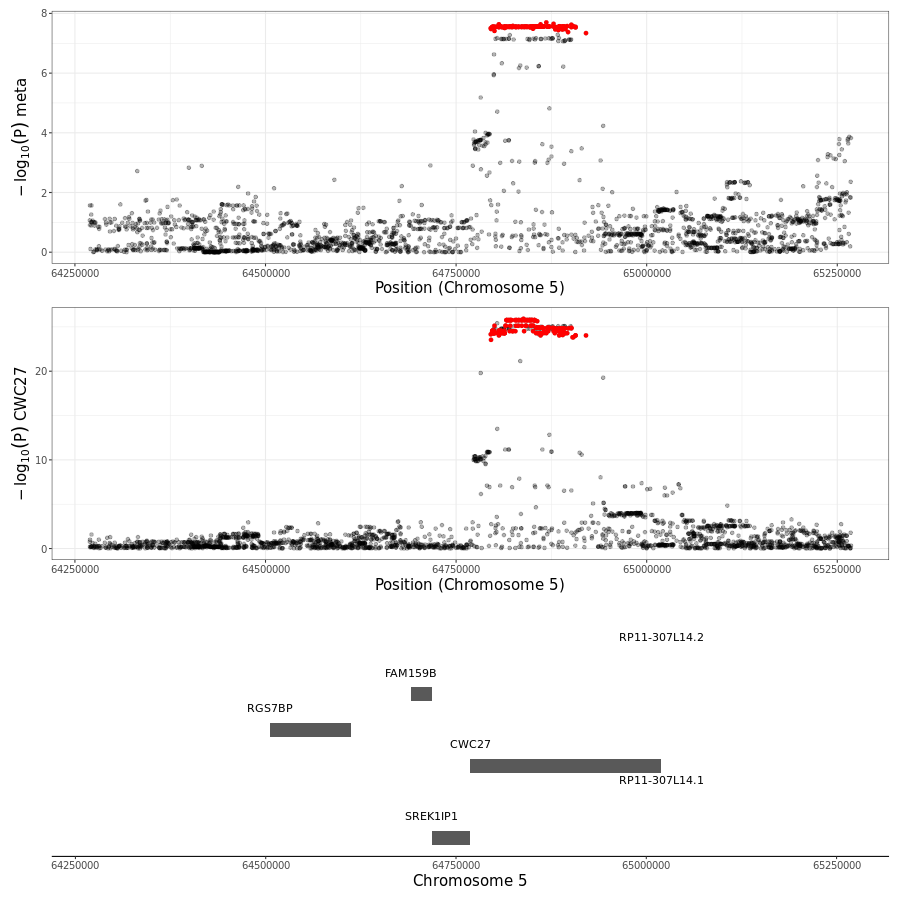
\includegraphics[width=1.0\textwidth]{Vector/cwc27_testis.png}
    \caption[Figure]{Regional association plot for the pAD-associated signal at index variant 5:64868326\_TTTC\_T (top) and \textit{CWC27} eQTL in testis (middle), showing position on the x-axis and $-log_{10}$ (P-value) on the y-axis. Red dots show pAD-associated genome-wide significant variants. Protein-coding and lincRNA gene positions are also shown (bottom).}
    \label{fig:cwc27_testis}
    \end{figure}





\section{Discussion}
In this chapter, I have performed several analysis to map genetic variants associated with perianal disease (pAD), defined as anal and rectal fissures and fistulas. I have leveraged two large-scale national biobanks, UKBB and FinnGen, with a total of 11,216 cases and 585,420 controls. First, I performed a separate UKBB GWAS and found seven genome-wide significant loci, that I subjected to a number of post-GWAS quality checks to ensure their veracity. Next, I downloaded FinnGen GWAS summary statistics for the same phenotype and performed similar post-GWAS quality checks. I also attempted to cross-replicate each GWAS' findings, and found that three of the seven UKBB loci replicated in FinnGen, while all FinnGen loci replicated in the UKBB. Interestingly, all the UKBB loci that failed to replicate in FinnGen were located in the MHC region, which is known to be highly polymorphic and exhibits complex LD patterns that tend to be population-specific. \\

There are several possible explanations for the absence of replication at the MHC loci. First, the four MHC loci discovered in the UKBB GWAS may simply be spurious associations. As I showed in Section \ref{sec:ukbb_postgwas}, association strength and $R^{2}$ were not correlated in at least two of the MHC loci, which suggests that the underlying LD strcuture does not match general population LD and may lead to spurious associations at these loci. This could possibly result from cryptic population stratification, but it could also result from poor genotyping or imputation. Second, it is possible that neither the index variants nor their LD friends tag the true causal variant in FE. This is likely to be the case for the MHC loci where the index variant tags few or no LD friends. Third, a lack of statistical power might lead to an absence of replication, especially given the heterogeneity in pAD cases. The UKBB pAD case cohort is composed of perianal fissure and fistula cases, with fistulas representing 37.7\% of the pAD cases and it is unclear whether the FinnGen case cohort composition is similar. \\

% In order to maximise power to detect more genome-wide association signals, I then performed a fixed effects meta-analysis between the two GWAS. FinnGen and UKBB are derived from two different populations, with different LD structures, and therefore any genome-wide significant loci need to be carefully assessed to ensure they conform that the association strength conforms to both constitutent populations. Following this check, I found 12 genome-wide significant loci, two of which were located in the MHC region. Additionally, none of the index variants at these loci showed evidence of heterogeneity of effects between the two cohrots.\\

% Despite the increased power afforded by meta-analysis, several limitations should be noted. First, a large proportion of the variants used in the meta-analysis (31\%) were either not genotyped/imputed or did not pass genotype or imputation QC in one of the two GWAS. This heterogeneity may bias which variants achieve genome-widen significant association, and may have led to missing several genome-wide significant hits. Second, pAD definition is based on a relatively broad ICD-10 code and a broad FinnGen endpoint that encompasses acute and chronic fissures and fistulas. The contribution of each of these subphenotypes to the genome-wide significant signals is not obvious. In this study, I was limited by the restricted access to individual-level FinnGen data, but future work should focus on assessing the contribution of each of the pAD subtypes to each genome-wide significant locus. \\

% , over the last several thousand years, Finnish Europeans were admixed with several Central Asian and East Asian populations, as well as Non-Finnish Europeans \cite{Qin2015-jb}. This admixture led to systematic differences between Finnish and Non-Finnish Europeans, both in terms of allele frequencies and LD strucure. Second,
Despite the increased power afforded by meta-analysis, several limitations should be noted. First, although case and control inclusion criteria are similar between the two cohorts, it is not obvious if the composition of the pAD case cohort is also similar. Similar to the ICD codes used in the UKBB analysis to identify anal fissures and fistula cases, FinnGen's clinical endpoint covers two broad clinical diagnoses: anal fissures and fistulas. I have shown in Table \ref{table:ukbb_level2_nums} that the proportion of anal fissures and fistula cases in the UKBB case cohort is roughly 2:1. Since FinnGen's individual-level data are not publicly available, I could not confirm if the proportion of anal fissure and fistula cases are similar. Second, it is unclear if FinnGen's case cohort is enriched in any other clinical endpoints compared to FinnGen's control cohort. Showing that the pAD cases are enriched in the same disorders (e.g. haemorrhoids and anal abscess) can serve as an important phenotypic quality control check to ensure that both cohorts are as similar as possible, and maximises the ability of a meta-analysis to identify genetic variants associated with pAD risk. In this study, I was limited by the restricted access to individual-level FinnGen data, but future work should focus on assessing the contribution of each of the pAD subtypes to each genome-wide significant locus.\\

% Following up on the meta-analysis results, I prioritised two follow-up analyses to better characterise the effects of the 12 pAD-associated loci. 

I observed that pAD cases are highly enriched in haemorrhoids compared to pAD controls (38\% versus 6\% respectively), which may suggest that there may be shared genetic effects underlying both pAD and haemorrhoids. I therefore performed an analysis where I disentangled the effects of the pAD-associated variants on both diseases. This analysis showed that the effects of these variants were stronger and more significant on pAD than haemorrhoids despite a large difference in statistical power in favour of haemorrhoids. However, this analysis was limited to UKBB participant, and it is plausible that better powered GWAS of haemorrhoids may reveal that a larger proportion of the 12 pAD-associated variants are also associated with haemorrhoids. Indeed, when I replicated the index variants in the largest haemorrhoids GWAS (Zheng et al. \cite{Zheng2021-ss}), I found that six of the 12 variants showed genome-wide significant association (P-value < $5\times10^{-8}$). However, similar to the UKBB analysis, they all had a concordant but smaller effect sizes on haemorrhoids than pAD. A compelling interpretation of this shared genetic risk is that pAD may be a more severe form or manifestation of haemorrhoids, with the same genetic variants underlying both and with stronger effect sizes on pAD. But this observation may not be true for all haemorrhoids-associated loci. Over 100 haemorrhoids-associated loci were identified by Zheng et al., and it is plausible that most of these loci will not be associated with pAD if a genome-wide significant comparison of effect sizes was performed between the two diseases. Therefore, any conclusions made regarding the difference in effect sizes should be limited to these 12 loci.\\

Finally, I aimed to identify effector genes at each locus using colocalisation analysis. Although I identified several genes that colocalised with high confidence, evidence at most loci was conflicting, implicating several genes in several tissues. The role of these genes in many of the tissues where the colocalistions were detected, such as testis, thyroid and liver, was difficult to interpret given our knowledge of the pathogenesis of pAD. Although I showed evidence that two of these genes, \textit{LFNG} and \textit{CWC27}, were necessary for normal skeletal development, this does not constitute sufficient evidence for a novel insight into pAD pathogenesis. To this end, more follow-up work should be conducted to better interpret these loci. First, more robust methods need to be employed to establish a causal link between these loci and effector genes (e.g. Mendelian Randomisation methods \cite{Sanderson2022-nm}). Additionally, QTL studies from more relevant tissues need to be used. As discussed in \ref{sec:coloc}, it is well-known that genetic variants affect the expression of different genes in different tissues. Therefore, QTLs derived from anorectal tissues will provide the best colocalisation and mendelian randomisation evidence for effector genes. However, the anal region is composed of several tissues and cell types, and it is plausible that colocalisation with single-cell QTLs derived from anorectal biopsies will also potentially implicate different genes in different cell types. Therefore, the first step to identify the most likely effector genes is to identify the most relevant cell type via a heritability enrichment analysis (e.g. LDSC-SEG \cite{Finucane2018-mx}). In conclusion, establishing a bona fide set of effector genes for these loci in relevant tissues will provide much stronger evidence that points to biological pathways implicated by pAD loci effector genes. 
